%%%%%%%%%%%%%%%%%%%%%%%%%%%%%%%%%%%%%%%%%%%%%%%%%%%%%%%%%%%%%%%%%%%%%%%%
% LaTeX template to generate an NSF proposal
%
% First version by: Stefan Llewellyn Smith, Sarah Gille, others.
%
% Additions by: Ronni Grapenthin, New Mexico Tech.
%
% This version maintained/modified by: Jeremy A. Gibbs, NOAA NSSL
%
% This template is free source code. It comes without any warranty, to
% the extent permitted by applicable law. You can redistribute it and/or
% modify it under the terms of the Do What The Fuck You Want To Public
% License, Version 2, as published by Sam Hocevar. See
% http://www.wtfpl.net for more details.
%%%%%%%%%%%%%%%%%%%%%%%%%%%%%%%%%%%%%%%%%%%%%%%%%%%%%%%%%%%%%%%%%%%%%%%%

%%%%%%%%%%%%%%%%%%%%%%%%%%%%%%%%%%%%%%%
% Package calls and title
%%%%%%%%%%%%%%%%%%%%%%%%%%%%%%%%%%%%%%%
%!TEX root =  proposal.tex

\usepackage[T1]{fontenc}
%\usepackage[latin1]{inputenc}
\usepackage[amssymb]{SIunits}
\usepackage{latexsym}
\usepackage{multirow}
\usepackage{wrapfig}
\usepackage{amsmath, amsthm, amssymb}
\usepackage{amsfonts}
\usepackage[format=plain,indention=0cm, font=small, labelfont=bf]{caption}
\usepackage{longtable}
\usepackage{fancyhdr}
\usepackage[pdftex]{graphicx}
\usepackage[pdftex,
	    colorlinks,
	    pdfstartview=FitH,
	    linkcolor=black,
	    citecolor=black,
	    urlcolor=black,
	    filecolor=black
	    ]{hyperref}
\usepackage{lscape}
\usepackage{floatrow}
%\usepackage{enumerate}
%\usepackage{enumitem}
\usepackage{tabularx}
\usepackage{ragged2e}

\usepackage[normalem]{ulem} % allows text to be striked out. use \sout{xxx}

% \definecolor{coolblack}{rgb}{0.0, 0.18, 0.39}
% \definecolor{darkcerulean}{rgb}{0.03, 0.27, 0.49}
% 
% \newcommand{\propose}[1]{{\color{darkcerulean}#1}}

\usepackage[table]{xcolor}
\usepackage{comment}
\usepackage{ifthen}

\newcolumntype{Y}{ >{\RaggedRight\arraybackslash}X}
\newcommand\T{\rule{0pt}{2.6ex}}
\newcommand\B{\rule[-1.2ex]{0pt}{0pt}}

\renewcommand{\refname}{References Cited}

\newcommand{\degrees}{$\!\!$\char23$\!$}

\def\rrr#1\\{\par
\medskip\hbox{\vbox{\parindent=2em\hsize=6.12in
\hangindent=4em\hangafter=1#1}}}

\renewcommand\baselinestretch{1}
%%% \pagestyle{empty}
%%% INCLUDE THE ABOVE TO PUT PAGE NUMBERS BACK IN

%\setlength{\parindent}{0pt}
\setlength{\parskip}{1ex}

%!TEX root =  proposal.tex

\usepackage[moderate,bibnotes,charwidths,mathdisplays,indent]{savetrees}

%\usepackage[textsize=tiny]{todonotes} % package for cool todonotes in the margin
%\usepackage[normalem]{ulem} % package that allows text to be striked out
\usepackage{titlesec}

\titlespacing*{\section}
{0pt}{2.5ex plus 1ex minus .2ex}{1.3ex plus .2ex}
\titlespacing*{\subsection}
{0pt}{2.5ex plus 1ex minus .2ex}{1.3ex plus .2ex}


\usepackage{amsmath}
\usepackage{amsthm}
\usepackage{amstext}
\usepackage{amsfonts}
\usepackage{mathrsfs}
\usepackage{xcolor}
\usepackage{tikz}
\usepackage{cleveref}
\usepackage{subcaption}
\usepackage{cite}
\usepackage{pgfplots}
\pgfplotsset{compat=1.3}
\usepackage{url}
\urlstyle{tt}
\usepackage{xspace}
%\usepackage{algorithm}
%\usepackage[noend]{algpseudocode}
%\usepackage{siunitx}
\usepackage{booktabs}
\usepackage{multirow}
\usepackage{comment}
\usepackage[title]{appendix}
\usetikzlibrary{external}
%\usepackage{enumitem}
\usepackage{balance}
\usepackage{pgfgantt}

\iffalse
\usepackage{xr}
% In your preamble

\makeatletter
\newcommand*{\addFileDependency}[1]{% argument=file name and extension
  \typeout{(#1)}
  \@addtofilelist{#1}
  \IfFileExists{#1}{}{\typeout{No file #1.}}
}
\makeatother

\newcommand*{\myexternaldocument}[1]{%
    \externaldocument{#1}%
    \addFileDependency{#1.tex}%
    \addFileDependency{#1.aux}%
}
\myexternaldocument{supplementary}
\fi



\usepackage{graphicx}

\usepackage{svg}

%\usepackage{amssymb}

%!TEX root =  proposal.tex


%% MAB: for proposing text
\definecolor{coolblack}{rgb}{0.0, 0.18, 0.39}
\definecolor{darkcerulean}{rgb}{0.03, 0.27, 0.49}
\newcommand{\propose}[1]{{\color{darkcerulean}#1}}

% MAB: this is the macro we can use to enumerate research problems
\newtheorem{eval}{Evalulation}
\newtheorem{prob}[eval]{Research Problem}
\newtheorem{rproblem}[eval]{Research Problem}
\newtheorem{proofofconcept}[eval]{Proof of Concept}

\newcommand{\evalref}[1]{Evaluation~\ref{#1}}
\newcommand{\evalreftwo}[2]{Evaluations \ref{#1} and~\ref{#2}}
\newcommand{\evalrefthree}[3]{Evaluations \ref{#1}, \ref{#2},             and~\ref{#3}}
\newcommand{\evalreffour}[4]{Evaluations \ref{#1}, \ref{#2}, \ref{#3},                   and~\ref{#4}}


\newcommand{\errbits}{\log (1/\epsilon)}
\newcommand{\opt}{n\errbits}
\renewcommand{\epsilon}{\varepsilon}

% \newcommand{\defn}[1]{\textit{#1}}
\newcommand{\defn}[1]{{\textit{\textbf{\boldmath #1}}}\xspace}
\newtheorem{theorem}{Theorem}
\newtheorem{lemma}[theorem]{Lemma}
\newtheorem{corollary}[theorem]{Corollary}
\newtheorem{claim}[theorem]{Claim}
\newtheorem{proposition}[theorem]{Proposition}
\newtheorem{assumption}[theorem]{Assumption}
\newtheorem{definition}[theorem]{Definition}
\newtheorem{invariant}[theorem]{Invariant}
\newtheorem{observation}[theorem]{Observation}

\ifdefined\textln\relax\else\newcommand{\textln}[1]{#1}\fi

%\makeatletter
%\algrenewcommand\ALG@beginalgorithmic{\footnotesize}
%\makeatother


\definecolor{magenta4}{rgb}{0.5625,0,0.5625}
\definecolor{green4}{rgb}{0,0.5625,0}
\definecolor{orange4}{rgb}{0.98,0.31,0.09}
\definecolor{powderblue}{rgb}{0.69,0.88,0.9}

\iftrue
\newcommand{\mab}[1]{{\scriptsize \textcolor{blue}{Michael: {#1}}}}
\newcommand{\mfc}[1]{{\scriptsize \textcolor{orange4}{Martin: {#1}}}}
\newcommand{\john}[1]{{\scriptsize \textcolor{pink}{John: {#1}}}}
\newcommand{\prashant}[1]{{\scriptsize \textcolor{cyan}{Prashant: {#1}}}}
\fi


% see http://latexcolor.com to define more colors

\newcommand{\fixme}[1]{\todo[size=\tiny]{#1}}

\newcommand{\TODO}{{\color{red}\bf TODO}}


\newcommand{\qf}{quotient filter\xspace}
\newcommand{\cqf}{counting quotient filter\xspace}
\newcommand{\bloom}{Bloom filter\xspace}
\newcommand{\btree}{B-tree\xspace}
\newcommand{\btrees}{B-trees\xspace}
\newcommand{\bplustree}{B$^+$-tree\xspace}
\newcommand{\bplustrees}{B$^+$-trees\xspace}
\newcommand{\proc}{\texttt}


\newcommand{\kmer}{$k$-mer\xspace}
\newcommand{\Kmer}{$K$-mer\xspace}
\newcommand{\kmers}{$k$-mers\xspace}
\newcommand{\Kmers}{$K$-mers\xspace}


\newcommand{\poly}[1]{\textrm{poly}{(#1)}}
\newcommand{\polylog}[1]{\textrm{polylog}{(#1)}}

\newcommand{\para}[1]{\smallskip\noindent\textbf{#1.}}

\newcommand{\punt}[1]{}

% \pagenumbering{gobble}
\renewcommand{\title}{\noindent {\textbf{A Compact, Dynamic, and Distributed Data
Structure Library for Computational Biology}}}

%%%%%%%%%%%%%%%%%%%%%%%%%%%%%%%%%%%%%%%
% Document starts here
%%%%%%%%%%%%%%%%%%%%%%%%%%%%%%%%%%%%%%%
\sloppy
\begin{document}

\newpage
\thispagestyle{empty}

%!TEX root =  proposal.tex

%% Don't actually need this - will submit txt.  Just want to estimate actual space
\begin{center}

\bf
\Large
Collaborative Research: CSR: Medium: \\Dynamic and Distributed Data Structures on the GPU

% \medskip
\small
Lead PI: Mart\'{i}n Farach-Colton (NYU) \\
Co-PIs: Michael A. Bender (SBU), John Owens (UC Davis), Prashant Pandey (Northeastern), Rob Patro (UMD)
\end{center}

\vspace{-0.3cm}
{\color{red}

\noindent \textbf{\large Overview:}\\
Both the volume and variety of genomic sequencing data has been increasing at an ever faster rate driven by high-throughput sequencing (HTS) technologies. 
% Genomic sequencing data is being generated faster than ever due to modern sequencing technologies.
% , which is already producing petabyte-scale datasets
Many applications in computational biology (\kmer analysis, single-cell transcriptomics, variant calling, transcript identification, raw sequence search, taxonomic classification, genome and metagenomic assembly, and pangenomics) require processing raw sequencing data at the petabyte scales.
%
These computational-biology applications (and numerous others) use a set of common data structures to perform many data-analysis tasks, and their performance is bottlenecked by the data-structure and algorithm performance.

This project aims to develop high-performance and scalable data analysis-pipelines for computational-biology applications. Specifically, we aim to develop new parallel and distributed data structures and algorithms that sit at the heart of many computational biology data processing tasks. These new data structures and algorithms will have wide applicability in computational biology applications and beyond.
%
We will develop new \textbf{algorithmic theory} to design scalable data structures and new \textbf{systems} that implement our solutions in a scale-up manner, both on CPUs and GPUs. We will develop a new framework to distribute our solutions in an \textbf{HPC} environment, so they scale out to clusters of GPUs; and finally we will validate our solutions on \textbf{computational biology} workloads.
%
Specifically, the data structures we propose to study are: \textbf{filters}, \textbf{sketches}, \textbf{hash tables}, \textbf{string indexes}, and related data structures.  We will validate our solutions on \textbf{large-scale raw sequence search}, \textbf{single-cell preprocessing}, \textbf{taxonomic classification for metagenomic data}, \textbf{pangenomic indexing and analysis}, \textbf{metagenome assembly}, and others.

\noindent \textbf{\large Keywords:} Data structures, algorithms, computational biology, GPUs, high-performance computing (HPC).

\noindent \textbf{\large Intellectual Merit:}\\
If successful we will be able to perform complex data analyses to answer biological questions on terabyte- and petabyte-scale datasets. For example, raw sequencing data from sequence read archive (SRA) is already at petabyte scale, metagenomic data from Western Arctic and Rhizo are in terabytes, and population-scale pangenomic data from the 100,000 Genome Project contains the genomes of $\approx85$K individuals. Existing data structures and software tools fail to scale to these data sizes, limiting the value of these essential public resources, and hampering critical data re-analysis in light of new and improved computational methods.

The project’s novelties are: a vertical-stack approach spanning \textbf{theory and algorithms}: highly concurrent, dynamic, and distributed data structures, \textbf{systems}: scale up using GPU acceleration, \textbf{high-performance computing}: scale out using distributed data structures, and \textbf{applications}: computational biology applications; new parallel and distributed data structures and algorithms to exploit the massive compute on GPUs applicable to other application domains; and an API for developers to quickly and seamlessly integrate high-performance and scalable data structures in applications.
%
Our team constitutes a highly interdisciplinary array of researchers across four focus areas: applications (computational biology), theory and algorithms, systems, and high-performance computing. The team is taking a holistic theory/systems/HPC/applications co-design approach to explore four tightly interconnected research modules. These research modules are structured from bottom-up across the computing stack.

\noindent \textbf{\large Broader Impacts: }\\
The primary broader impact of this work is to enhance the capability of bioinformatics applications to perform computations at the largest scales. Both accelerated computation (allowing quicker feedback and more experiments) and larger computation potentially accelerate the process of scientific discovery. Second, we expect that a high-quality library of distributed, scalable GPU data structures will find widespread utility in other application domains.
%
Beyond technical broader impacts, we propose outreach impacts through tutorial on using our data structure library in computational biology conferences and proposing week-long research seminars like Dagstuhl that we hope will bridge the gaps between computational biologists, CS theorists, and CS systems researchers.
}

\newpage
\setcounter{page}{1}
%!TEX root =  proposal.tex


%%%%%%%%%%%%%%%%%%%%%%%%%%%%%%%%%%%%%%%%%%%%%%%
% These are the general sections to include.  %
%                                             %
% You can alter some names, but follow the    %
% suggestions in the NSF guidelines.          %
%                                             %
% If spacing is tight, play with negative     %
% vspaces w/in the text to reduce whitespace. %
%%%%%%%%%%%%%%%%%%%%%%%%%%%%%%%%%%%%%%%%%%%%%%%

%%%%%%%%%%%%%%%%%%%%%%%%%%%%%%
% Section 1: Introduction    %
%%%%%%%%%%%%%%%%%%%%%%%%%%%%%%
\section{Introduction}
\label{intro}


% \subsection{Problem}

% \mab{proposal format has too much white space between paragraphs...}

% MAB: the problem

Raw sequencing data in computational biology is increasing faster than ever
due to high-throughput sequencing technology (HTS), which is already producing
petabyte-scale datasets~\cite{kodama2012sequence}. Many applications in computational biology (\kmer
analysis~\cite{MarccaisKi11}, raw sequence search~\cite{SolomonKi16}, taxonomic classification~\cite{wood2014kraken}, and pangenomics~\cite{computational2018computational})
require processing raw sequencing data at petabyte scales~\cite{kodama2012sequence}. This project aims to
build high-performance and scalable data analysis-pipelines for computational-biology applications.
Specifically, we aim to develop new massively-parallel and distributed data structures and algorithms for core computational biology data processing tasks.


We aim to develop new data structures and algorithms that will have wide applicability in computation biology and beyond. For concreteness, we consider the following tools that are used throughout computational biology.

\begin{itemize}[leftmargin=*]

\item {\bf \Kmer analysis.}
\Kmer analysis involves representing raw sequencing data as length-$k$ subsequences called \kmers, and performing analysis on the occurrence and frequency of \kmers in the data sets; the objective is to answer questions about the genomic diversity, abundance variance, taxonomic information, etc. \Kmer analysis is the first step in numerous computational-biology pipelines, e.g., error correction, de Bruijn graph construction, raw sequence search, digital normalization, comparative genomics, genomics assembly, transcript quantification, taxonomic classification of metagenomic reads, etc~\cite{wood2014kraken,GeorganasEHG18,hofmeyr2020terabase,solomon2016fast,PatroSailfish:2014,PandeyABFJP18Cell,PandeyBJP17a,PandeyBJP17b}.

Existing tools use both  approximate\footnote{In this proposal, we refer to data structures as approximate if they only have false positives and lossy if they have false negatives.} and exact data structures (e.g., filters vs.\ hash tables) to construct and store \kmer indexes~\cite{MarccaisKi11,PandeyBJP17a}.  \kmer analysis tools such as  Jellyfish~\cite{MarccaisKi11} use a compact filter to identify singleton \kmers and use a hash table to maintain the frequency count and associated metadata (e.g., prefix-suffix extension, read id, etc) about the \kmers~\cite{HofmeyrEGC20}.

As we will see, \kmer analysis is a part of several of the specific applications we will be addressing.

% \item {\bf Compressed indexes.}
% FM-index, BWT, comressed suffix array.

\item {\bf Sequence alignment.} Sequence alignment involves aligning sequences of DNA, RNA or protein to identify similar regions that may be a consequence of underlying biological process and to establish evolutionary relationships.
Sequence alignment is extensively used in the genomic and metagenomic assembly process to map the contigs back to the input raw reads to extend the contigs in the correct order to construct the full genome. In computational-biology applications, sequence alignment is often performed sequence to sequence; between multiple sequences (\emph{multiple sequence alignment}); and from a sequence to graph where the the graph is a sequence graph representing genomes from multiple individuals.

Existing tools use compressed and succinct string indexes such FM-index~\cite{ferragina2000opportunistic}, BWT~\cite{burrows1994block}, compressed suffix arrays~\cite{grossi2000compressed} and dynamic programming algorithms for sequence alignment.
Compressed and succinct indexes help to perform sequence alignment in a memory-efficient manner and enable these tool to scale to large-scale sequencing data.
One of the most widely used tools across computational biology, BLAST~\cite{altschul1990basic}, performs fast and efficient sequence alignment using compressed string indexes.
Given the large sizes of sequencing datasets, these tools also use hash-based \kmer indexes to seed the sequence alignment to achieve speed ups.


\end{itemize}

This toolbox is used, for example, to solve the following problems.

\begin{itemize}[leftmargin=*]

\item {\bf Taxonomic classification.} Taxonomic classification~\cite{wood2014kraken} helps to identify the microbial taxon or taxa present in large-scale  metagenomic datasets coming from complex biological and environmental samples. Assigning taxonomic labels to sequencing reads is an important part of many computational genomics pipelines for metagenomics projects.

Methods for taxonomic classification of metagenomic data~\cite{wood2014kraken} often use hash tables to index the \kmer content of samples and quickly compare samples to prune down the search space.
Furthermore, to save space many solutions~\cite{wood2019improved} also employ approximate sketches (e.g., locality sensitive hashing (LSH)~\cite{roberts2004reducing}) to represent metagenomic data and perform similarity computations over sketches.
They further employ compact string indexes such as FM-index~\cite{ferragina2000opportunistic} and compressed suffix array (CSA)~\cite{grossi2000compressed} to perform sequence comparison to determine exact matches among the pruned-down samples.


\item {\bf Raw sequence search.} Raw sequence search involves  identifying all sequencing samples in a database of raw sequencing data such as SRA~\cite{kodama2012sequence} that contain a given query sequence. A query is an arbitrary sequence, such as a transcript. Raw sequencing datasets contain a ton of biological diversity information that can be used to answer biological questions that single sequencing sample do not have the power to address.

Methods for raw sequence search use \kmer-based indexing tools to build an inverted index from the \kmers to the underlying samples the \kmer is present in. Tools like SSBT~\cite{SolomonKi16} build a tree of approximate \kmer indexes to quickly prune down the search space of sample. While Mantis~\cite{PandeyABFJP18Cell} build an exact inverted index using compact hash tables.
In raw sequencing data, singleton \kmers are most likely caused by sequencing errors, yet they make up a large fraction of the data~\cite{solomon2016fast,MarccaisKi11}. These tools often use filters to weed out singleton \kmers.


\item {\bf Pangenomics.}
Pangenomics~\cite{garrison2018variation} involves storing the genome of a species as a sequence graph consisting of genomes of multiple individuals instead of a single linear reference. A primary goal of pangenomic variation analysis is to avoid biases that arise when treating a single genome as the reference when identifying or comparing variants across samples in a population.

Existing tools for constructing a pangenomic graph use a combination of succinct data structures (e.g., compressed bit vectors~\cite{garrison2018variation}), space-efficient, dynamic hash tables, and string data structures~\cite{pandey2021variantstore}.

\end{itemize}

Our goal is to build tools to perform complex biological analyses at terabyte and petabyte scale to explore datasets available today and expected to be available in future. For example, raw sequencing data from SRA~\cite{kodama2012sequence} is already at petabyte scale, metagenomic data from WA and Rhizo~\cite{hofmeyr2020terabase} are hundreds of terabytes, and pangenomic data from 100,000 genome project~\cite{1002021100} are sequencing individuals at population scale. To quickly process and perform biological analysis on these data we will exploit the massive computing in modern GPUs (V100 and A100) and also the distributed computing infrastructure of super computers (Perlmutter~\cite{perlmutter} and Summit~\cite{summit}).




The computational-biology applications described above (and numerous others)  use a set of common data structures to perform data-analysis tasks.
Compact and exact data structures include: hash tables and succinct bit vectors, compressed string indexes, trees.
Sketches and approximate data structures include: filters, cardinality estimators,  min-hash based sketches, other locality-sensitive hash data structures.

The performance and scalability of the computational-biology applications
depends on the space-efficiency, speed, dynamism, and scalability of the
underlying data structures they use. These data structures are also the building
blocks in many other domains, such databases, machine learning, software
systems, security applications, etc.


% \setlength\intextsep{0pt}
\begin{wrapfigure}{R}{0.75\textwidth}
% \begin{figure}
\centering
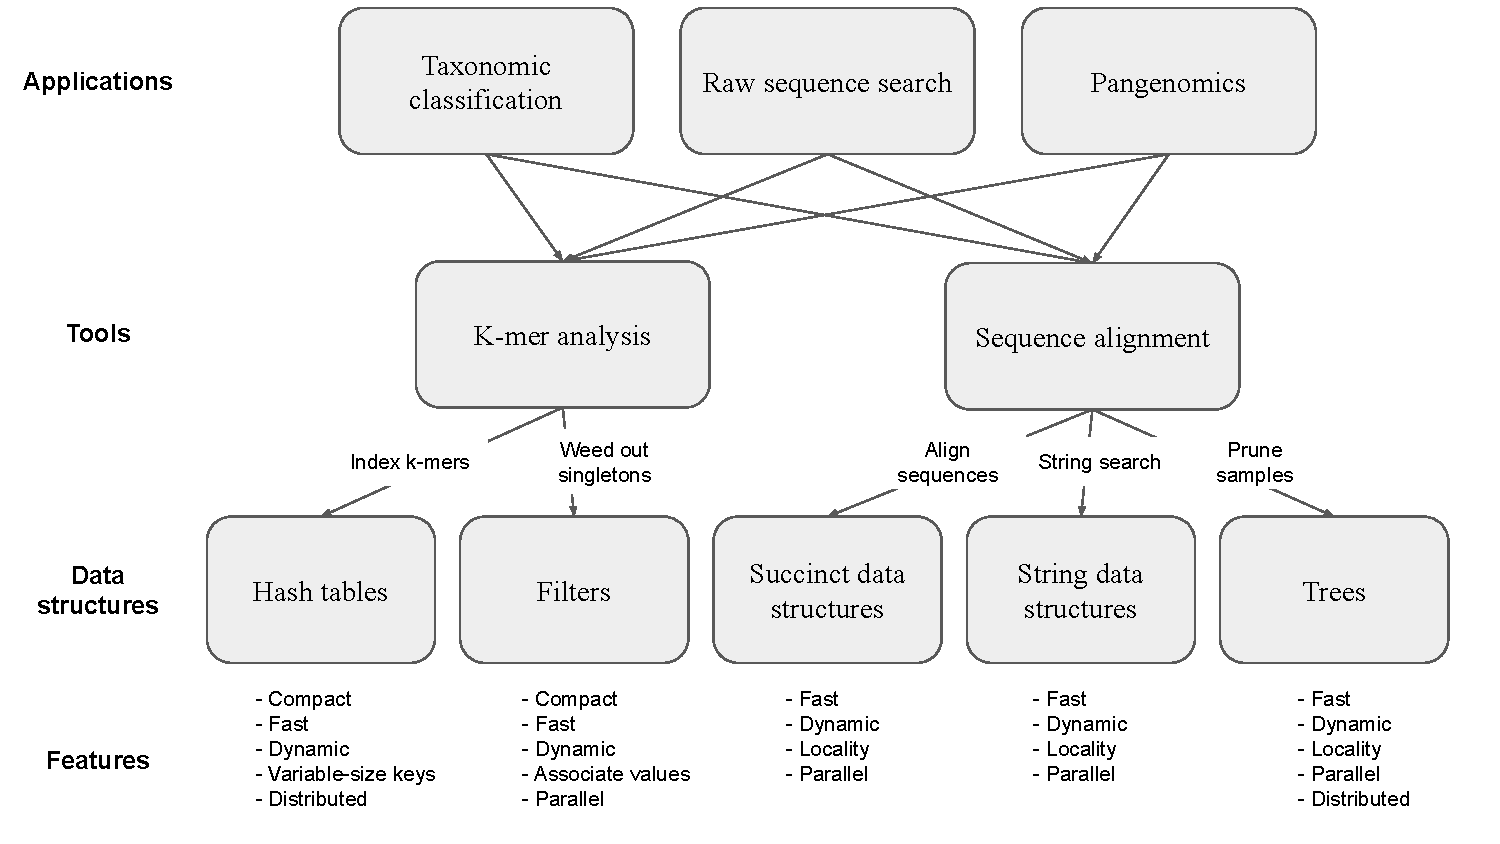
\includegraphics[width=0.9\textwidth]{images/PPOSS_App_DS}
\caption{Relation between computational-biology applications, data processing tools and data structures. We further mention the desired features in data structures to achieve performance and scalability.}
\label{fig1}
% \end{figure}
\end{wrapfigure}


\paragraph{Existing software tools for computational-biology applications.}

There are numerous tools for \kmer counting~\cite{MarccaisKi11,PandeyBJP17a}, sequence alignment~\cite{altschul1990basic,kielbasa2011adaptive,li2018minimap2,schwartz2003human}, raw sequence search~\cite{solomon2016fast,PandeyABFJP18Cell}, taxonomic classification~\cite{wood2014kraken,wood2019improved}, and pangenomics~\cite{garrison2018variation,pandey2021variantstore}. These tools rely on space-efficient and high-performance CPU data structures such as filters, sketches, hash tables, and string indexes. Most of these tools are designed for shared-memory parallelism and they often do not scale out of shared memory to disks.
These existing tools are limited by the single-node compute and shared-memory parallelism. They are not designed to scale to thousands of core on modern accelerators and scale out to hundreds to nodes in a high-performance computing (HPC) environment.
%
\prashant{I don't like the above paragraph much...}

% \begin{wrapfigure}{r}{0.4\textwidth}
% \centering
% 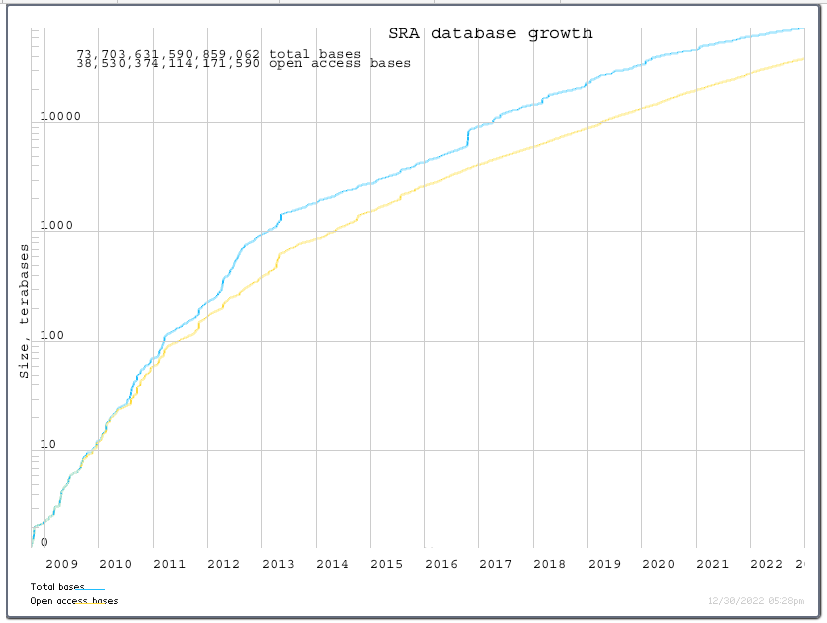
\includegraphics[width=0.95\textwidth]{images/SRA_data_growth.png}
% \caption{Sequence read archive (SRA) data growth. SRA data contains a trove of biological diversity information. Existing computational-biology tools do not scale to support searching through all of SRA. This renders what is otherwise an immensely valuable public resource largely inert.}
% \label{fig:sra_data}
% \end{wrapfigure}

\label{sec:we-need-performance-and-scalability}
\paragraph{CPU speed and RAM capacity cannot keep up with data growth.}
Unfortunately, CPU speed and RAM sizes aren't keeping up with the data growth in computational biology and other applications.
Although CPUs are increasing at 2--25\%/year and single-node RAM sizes are increasing at 2-11\%/year, genomics data is is likely to double in size every $1.5$ years~\cite{kodama2012sequence}.
Thus, today's software tools will not scale with tomorrow's data. For example, performing \kmer analysis or sequence alignment on petabyte-scale raw sequencing data is not possible on single-node shared-memory systems.

As mentioned by Leiserson et al.~\cite{leiserson2020there}, in the post Moore’s law period the performance gains will come from software, algorithms, and hardware (referred as the top of the computing stack) rather than the semiconductor (referred as the bottom). We can achieve massive scalability by, first designing data structures and algorithms to scale up using modern accelerators such as GPUs and second scaling out by using distributed memory in an high-performance computing (HPC) environment.


\paragraph{GPUs and other accelerators in computational biology.}
As with other high-performance computing (HPC) domains,
GPUs are increasingly used in large-scale computational biology because they offer orders of magnitude of jump in terms of low-cost parallelism, as long as data structure and algorithms can be defined to conform to the memory and parallelism requirement of GPUs.
%
For example, GPUs are used in some computational-biology applications to speed up \kmer counting~\cite{nisa2021distributed} and local assembly~\cite{awan2021accelerating}.
\prashant{Check if there are more examples.}

However, the penetration of GPUs into biology pipelines is limited by how the limitations of GPUs have translated so far into data structures.  These GPU limitations include:
\begin{enumerate}[noitemsep,nolistsep]
  \item GPU device RAM is much smaller than CPU RAM; this is especially
    challenging given the data sizes in computational biology.
  \item GPUs have high contention due to thousands of threads and are
    inefficient when computations are irregular.
  \item GPUs don't have a memory system; it is hard to perform dynamic memory management without involving the host CPU.
\end{enumerate}

These limitations affect the capabilities of GPU data structures: most existing GPU data structures do not support dynamic resizes and are statically allocated; pointer-based data structures such as trees and tries do not achieve high performance on GPUs; data structures on hard-to-align data, such as string or vectors, which have variable lengths are not available; data structures do not scale out of GPU device RAM to host.

These limitations are critical for building scalable computational-biology applications. For example, in \kmer analysis during raw sequence search and taxonomic classification the size of the \kmer multiset is not known in advance. Therefore, applications initialize the data structures such filters and hash tables to a default size and then dynamically resize (mostly expand) based on the actual number of \kmers. The ability to resize is critical to perform \kmer analysis in a space-efficient manner. Static data structures such as the hash tables and filters~\cite{GeilFO18} currently available on GPUs are sized using an over approximation of the number of \kmers which leads to space inefficiency.
Similarly, the local assembly module involves constructing thousands of hash tables in parallel and then using those hash tables to perform contig (contiguous strand of DNA) extension walks. The CPU implementation of local assembly relies heavily on dynamic
structures like hash tables, vectors and strings, which are a challenge to implement on GPUs. In addition, the algorithmic motif of local assembly induces a random memory-access pattern with a non-deterministic amount of work, which makes implementing this module on GPUs a very challenging problem.



% GPUs have not seen widespread adoption in computational biology applications. For example, they are used in taxonomic classification of metagenomic data, indexing and searching through terabytes of raw sequencing data, constructing and querying pangenomic graphs.

%Anything that involves sophisticated data structures and when memory is constrained GPUs are not currently useful.

% GPUs are not currently used for many computational biology applications because efficient GPU data structures do not exist.

\paragraph{Requirements for building scalable computational-biology applications}

Data structures are the core of computational-biology applications and are critical for their performance and scalability.
To build scalable computational-biology applications that can keep up with the rapid growth data we need compact, high-performance, dynamic, and distributed data structures. Specifically, we need: approximate data structures such as filters, sketches, and locality-sensitive hashing data structures; exact data structures such as hash tables, string data structures, succinct data structures, and trees.

These data structures and algorithms will need to exploit accelerators such as GPUs to scale up computations and at the same time support  features like space-efficiency, dynamism, high concurrency, scaling out of GPU device RAM to host RAM, and distributed memory design to scale out to multiple nodes.
%
Furthermore, to achieve fine-grained resizing and to keep the peak memory usage low we first need to develop new algorithmic approaches for traditional CPU data structures and then extend them to GPUs.

\subsection{Our proposed work}

We believe the answer to these challenges is a standalone library of memory-efficient, high-performance, dynamic, and scalable GPU data structures that can be directly used by computational biology applications that addresses the needs of emerging applications, allowing them to solve the problems described above.

\paragraph{Our approach is four-pronged.}  We will develop new \textbf{algorithmic theory} to design scalable data structures; we will develop new \textbf{systems} that implement our solutions in a scale-up manner,  both on CPU and GPU; we will a new framework to distribute our solutions in an \textbf{HPC} environment, so they  scale out to clusters of GPUs; and finally we will validate out solutions on \textbf{computational biology} workloads.
%
Specifically, out data structures are: \textbf{filters}, \textbf{hash tables}, \textbf{string indexes}, \textbf{sketches}, and related auxialiary data structures.  We will validate our solutions on \textbf{large-scale raw sequence search}, \textbf{taxonomic classification for metagenomic data}, \textbf{pangenomic indexing and analysis}, and others.

If successful we will be able to perform complex data analyses to answer biological questions on terabyte and petabyte scale datasets available. For example, raw sequencing data from SRA~\cite{kodama2012sequence}, metagenomic data from WA and Rhizo~\cite{hofmeyr2020terabase}, and pangenomic data from 100,000 genome project~\cite{1002021100}. Existing data structures and software tools fail to scale to the data sizes making a these publicly-available and highly-valuable data resources largely inert.


The project’s novelties are: a vertical-stack approach spanning theory and algorithms: highly-concurrent, dynamic, and distributed data structures, systems: scale up using GPU acceleration, high-performance computing: scale out using distributed data structures, and applications: computational biology applications; new parallel and distributed data structures and algorithms to exploit the massive compute on GPUs applicable to other application domains; an API for developers to quickly and seamlessly integrate high-performance and scalable data structures in applications.
%
Our team includes a highly interdisciplinary team of researchers across four focus areas: applications (computational biology), theory and algorithms, systems, and high-performance computing. The team is taking a holistic theory/systems/HPC/applications co-design approach to explore four tightly interconnected research modules. These research modules are structured from bottom-up across the computing stack.


% \paragraph{Roadmap.} Roadmap here. In Section

% Section 2: bioinformatics problems, state of the art, what we need

% Section 3: Our approach: Why GPUs?  Also GPU-specific generic research problems

% Section 4: Filters, with reserach problems -- theory, systems, HPC

% Section 5: Hash tables, with reserach problems -- theory, systems, HPC

% Section 6: String indexes, with reserach problems -- theory, systems, HPC

% Section 7: Sketches, with reserach problems -- theory, systems, HPC

% Section 8: Bioinformatics validation, with research problems for each bioinformatics problem, and if successful statements.

\iffalse
==========



\begin{itemize}[noitemsep, leftmargin=*]
  \item {\bf Module 1 [theory/algorithms]:} Develop single-node GPU data structures.
    Specifically, filters, hash tables, succinct/string data structures, and
    trees. Challenges: high concurrency; being able to scale 100K threads;
    branching statements have a high cost; data movement and irregular data
    accesses are expensive. We will develop new theoretical data structures and
    algorithms that can efficiently exploit massive GPU parallelism while being
    compact and dynamic.

  \item {\bf Module 2 [Systems]:} Develop GPU data structures that can scale out of
      GPU device RAM to CPU host RAM. We will develop a memory allocator to
      seamlessly manage the GPU and CPU ram and efficiently move data across GPU
      and CPU RAMs.

    \item {\bf Module 3 [HPC]:} Develop data structures that can scale out to
      multiple-GPU nodes in a distributed computing environment. We will develop
      communication-efficient distributed versions of the above data structure
      to efficiently scale out hundreds of nodes in a HPC environment.

    \item {\bf Module 4 [Applications]:} Building high-performance and scalable
      computational biology applications by integrating GPU data structures in
      k-mer analysis, taxonomic classification, pangenomics tools.

\end{itemize}

-------------------------------------------------------------

In this project, we propose to develop a  collection of
memory-efficient, high-performance, dynamic, and distributed GPU data structures.
We will show how to use these data structures for our target applications in computational biology, as well as some others.
With the help these data structures, we aim to scale computational biology applications to massive datasets (raw sequencing datasets, metagenomic datasets from complex microbiomes, population-scale pangenomic datasets) and enable them to answer complex biological questions that are not possible today.
Because many of these applications require the same set of data structures, we will incorporate these data structures into a standalone library to enable easy reuse in other applications.

The PIs and others have shown that recent data structure advances~\cite{cite-somethin} show that
implementations that go beyond primitive data structures are possible on GPUs
but this work has not had much practical impact to date. \mfc{this is a big turd in teh middle of our first page -- well maybe the end of the first page -- is it even true? My papers with John are wracking up citatoins}    \mfc{awkward transition.  this is not about what we are proposing.  this comes before what we are proposing $\rightarrow$} A pure GPU solution is
desirable because transfer costs are high, and this is the direction being taken
in other application domains (machine learning, data science).

\paragraph{GPUs and other accelerators.}

In this project we envision solving these problems with a combination of  scale-up (via better algorithms and accelerators) and scale-out (distributing data and compute across multiple nodes of large high-performance computing systems). \mfc{how do you scale out without better algorithms?  you make it sounds like scaleup needs algorithms but any old crap will work for scaleout.  I don't think taht's true.}

% The rate of growth data is much higher than the growth of the CPU speeds and single-node storage capacities. CPU growth will not keep up with application demands.

Most existing applications in computational biology use CPUs to perform data  analysis.
However, the growth of the CPU speed and capacity is slowing and at the same time data is growing faster than ever. CPU growth will not keep up with application demands.

As a consequence, a few recent tools~\cite{cite-something} have tried to scale
up using accelerators like GPUs to speed up computations. However, these tools
use only primitive data structures and as a result achieve suboptimal
performance. Some applications [cite] have also tried to scale out using
distributed memory.  However, these applications are still limited by the CPU
speed and capacity and leave performance on the table due to suboptimal
scalability of data structures.


\prashant{Assigned to Martin/Michael: Need to add theory/algorithmic challenges
to develop GPU data structures. Why is it hard to just port existing CPU data
structures to GPUs.}


\begin{enumerate}[noitemsep, leftmargin=*]
  \item Filters
  \item Hash table
  \item String data structures (suffix array, FM index, BWT)
  \item Succinct data structures (Dynamic rank-select indexes)
  \item Trees and Tries
\end{enumerate}

\prashant{Martin, Michael wants a postdoc in year 3-4-5. Maybe a PhD student from John/Prashant.}


\prashant{Section 2: State of the art, data structures (theory/systems), applications. What are the deficiencies.}\\
\prashant{Section 3: Here's what we will do. Need a concrete plan with what we are going to. Sub-problems, milestones, schedule. How the four pillars interact.}\\
\prashant{Conclusion, Broader impact, previous NSF support}


%%%%%%%%%%%%%%%%%%%%%%%%%%%%%%
% Section 4: Management Plan %
%%%%%%%%%%%%%%%%%%%%%%%%%%%%%%
\section{Time Line and Management Plan}

\begin{table}[H]
\label{table1}
\renewcommand{\arraystretch}{0}
\caption{Project schedule.  PIs are Person One (P1), Person Two (P2), graduate student is GS, and the undergraduate student is US\@. Time frame gives the year each activity will occur.}
\scriptsize
\begin{tabularx}{\textwidth}{Y c c }
\hline
\hline
\textbf{Research Activity} & \textbf{Personnel} & \textbf{Time Frame}\\
\hline
Perform a task that sounds impressive & P2, US & Y1 \T\\
Perform another super-amazing task & P1, US & Y1 \T\\
Perform something else that may not be as sexy as the other things & P2, GS & Y1 \T\\
Wonder why you are such a terrible programmer & P1, US & Y1 \T\\
Analyze the results and stuff & P1, P2, SS & Y1,Y2 \T\\
Take the day off and grill some meat & P1, P2, SS & Y1,Y2 \T\\
Present findings at scientific meetings and publish results in peer-reviewed journals & P1, P2, US, GS & Y1, Y2, Y3\T\B\\
\hline
\hline
\end{tabularx}
\end{table}

\fi

\section{Research areas}

% The Project Description must contain a section titled "Research Areas" that must:

% Explicitly state and motivate at least four research areas covered (along with senior personnel with commensurate expertise);
% Describe the targeted distributed applications and systems, and the heterogeneous platforms on which they run; and
% Define relevant notions of scale and describe how scalability will be theoretically and experimentally evaluated for the targeted distributed applications and systems and heterogeneous platforms in (2) with respect to the full hardware/software stack.



\paragraph{Coverage areas.}
Data structures are ubiquitous throughout the hardware/software stack, as a way to build scalable computational biology applications that can process petabyte-scale genomic data.
Data structures have become a bottleneck, but redesigning data structures for GPUs to exploit massive parallelism and scaling to distributed memory is tantamount to renegotiating the division of labor among system components---requiring a closely knit team and an approach that weighs the costs and benefits holistically.
Our team has extensive expertise in the following four research areas:

% \begin{itemize}[noitemsep,nolistsep]

\begin{description}[noitemsep,nolistsep]
    \item[Theory and Algorithms (PIs Bender, Farach-Colton, Pandey and Patro)]
    Bender, Farach-Colton, Pandey and Patro have written numerous theory related publications and have made significant contributions towards designing efficient data structures and building scalable applications using their theoretical contributions~\cite{BenderFaGo18,BenderFaJo12,PandeyBJ17,PandeyABFJP18Cell,PandeyBJP17a,PandeyBJP17b,ConwayFaSh18,JannenYuZh15a,JannenYuZh15b,YuanZhJa16,pandey2021terrace,pandey2021variantstore,pandey2022iceberght,Assadi2023,Bender2023,pandey2020timely,PandeyCDBFJ21,mccoy2022high,Almodaresi2018Pufferfish,fan2023spt,Khan2021,Khan2022,Khan2023CapsSA,fan2023fulgor,Pibiri2023MacDBG}.

    \item[GPU Systems (PIs Owens and Pandey)] Owens's research program in GPU computing~\cite{Owens:2007:ASO,Owens:2008:GC} spans nearly 20 years and includes representative research advances in fundamental algorithms~\cite{Sengupta:2007:SPF}, data structures~\cite{Lefohn:2006:GGE,Alcantara:2009:RPH}, % scalability to multiple GPUs~\cite{Stuart:2009:MPO,Stuart:2011:EMT,Stuart:2011:MMO,Pan:2017:MGA,Pan:2018:SBS,Chen:2022:SIP},
    performance engineering~\cite{Zhang:2011:AQP}, programming models~\cite{Gupta:2012:ASO, Tzeng:2010:TMF}, and applications~\cite{Wang:2017:GGG}. Pandey's research includes building massively parallel and feature-rich GPU filters~\cite{mccoy2022high} and distributed-memory GPU hash tables for efficiently processing genomic data~\cite{nisa2021distributed}.

    \item[High-Performance Computing (PIs Bender, Farach-Colton, Owens, and
        Pandey)] Bender and collaborator Cindy Phillips have
      written a number of top-tier related papers in HPC~\cite{pandey2020timely,bender2017two,eckstein2015pebbl,agrawal1989four,bender2008communication,greenberg1999enabling},
      and had considerable impact on HPC practice.
      PI Bender's and Phillips's work in HPC has focused on scheduling and  won a joint R\&D 100 Award for processor scheduling and allocation algorithms, which were licensed by Cray and incorporated into SLURM\@.  PIs Bender and Farach-Colton's company Tokutek deployed software to manage metadata in a large cloud storage service. Owens led the first implementation of MPI on GPUs~\cite{Stuart:2009:MPO:withouturl,Stuart:2011:EMT}, the first multi-GPU MapReduce~\cite{Stuart:2011:MMO}, and more recent work on scalable graph analytics on HPC machines~\cite{Pan:2018:SBS,Pan:2017:MGA,Chen:2022:SIP}. Pandey has built the first GPU-based distributed-memory \kmer analysis pipeline for the MetaHipMer metagenome assembler~\cite{nisa2021distributed}.

    \item[Large-scale computational biology (PIs Bender, Farach-Colton, Pandey and Patro)] Pandey and Patro's work in computational biology has focused on rebuilding key parts of genomic, transcriptomic, and pangenomics analysis tool-chains around data structures and algorithms of their design, and have been having tremendous impact in the field. This work is described in flagship computational biology conferences (RECOMB, ISMB, WABI) and journals (Cell Systems, Genome Biology, Bioinformatics, JCB, Nature Biotechnology and Nature Methods)~\cite{PandeyABFJP18Cell,PandeyBJP17a,PandeyBJP17b,AlmodaresiPFJP19,AlmodaresiPFJP20,pandey2021variantstore,almodaresi2017rainbowfish,almodaresi2022incrementally,PatroSailfish:2014,Patro2017Salmon,Srivastava2019,he2022alevin,Almodaresi2018Pufferfish,Almodaresi2021}.  PI Farach-Colton has papers in genome assembly~\cite{Choi2003}, phylogeny construction~\cite{Farach97,Ambainis97,FarachKKM97,Farach1999, Cohen1997}, and string indexes~\cite{Farach97,Ambainis97}.

\end{description}


\paragraph{Notions of Scale.}
Our proposed work addresses several notions of scale.
% First, multi-core parallelism on CPUs is critical to efficiently scale data structure to exploit CPU compute.
First, our work involves scaling up data structures by designing them for GPUs. GPUs are cost-effective and offer massive parallelism, allowing significant speedups compared to CPUs. GPU data structures can help speed up computational-biology applications
% by orders of magnitude \john{this phrase ``orders of magnitude'' makes me nervous, I don't want to make reviewers nervous}
and quickly analyze large-scale datasets. Without a principled redesign of data structures, additional device RAM and GPU cores will be of diminishing value.
Second, our work includes scaling out data structures in distributed memory across multi-node GPUs to quickly process petabyte-scale genomic and metagenomic datasets. This will involve building distributed data structures that can offer low communication volume and low load imbalance. Prior work has demonstrated that data movement and load imbalance is the major bottleneck for achieving high performance in a distributed application.
Furthermore, computational biology datasets available today are already terabyte- and petabyte-scale. For example, raw sequencing data from SRA~\cite{kodama2012sequence}, metagenomic data from WA and Rhizo~\cite{hofmeyr2020terabase}, and pangenomic data from the 100,000 Genome Project~\cite{1002021100}. 
% \john{Pretty sure the previous sentence was already stated in the intro.} 
% \prashant{Yeah, Martin/Michael mentioned to repeat this a couple of times.}
To quickly process and perform biological analysis on these data, we need to exploit the massive computing in modern GPUs (V100 and A100) and also the distributed computing infrastructure of supercomputers (Perlmutter~\cite{perlmutter} and Summit~\cite{summit}).

%!TEX root =  proposal.tex

\section{Computational biology applications}


\subsection{Taxonomic classification of metagenomic data}

\textbf{Problem definition.}
The microbes that live in an environment can be identified by their combined genomic material, also called the metagenome.
The study of metagenomes provides an opportunity to closely examine complex biological interactions, such as phage-host and metabolic dynamics~\cite{national2007new}.
Metagenomic datasets contain sequencing reads from multiple species that are present in the biological environment.
%
Taxonomic classification~\cite{wood2014kraken} helps to identify the microbial taxon or taxa present in large-scale  metagenomic datasets coming from complex biological and environmental samples. Assigning taxonomic labels to sequencing reads is an important part of many computational genomics pipelines for metagenomics projects.

\noindent
\textbf{Importance.}
Metagenomic sequencing produces genomic data from a set of species instead of a pure species isolate. One of the primary challenges in the field is the development of computational methods for identifying all of the species contained in these samples.
%
Taxonomic classification of reads is a critical first computational step in any metagenomic analysis pipeline.
For example, read classification is critical for \emph{de novo} metagenomics assembly, which attempts to reconstruct the DNA sequence of each organism present in the metagenomic sample without using a reference database before performing the actual assembly step~\cite{venter2004environmental,brady2009phymm,brady2011phymmbl,rosen2008metagenome,segata2012metagenomic}.

\noindent
\textbf{Challenges.}
The task of read classification is far from straightforward.
A metagenomic sample can contain thousands of genomes with varying level of similarities and often occurring at vastly different abundances. Furthermore, due to high-throughput sequencing, metagenomic samples contain millions of sequencing reads making traditional, string-matching-based tools like BLAST~\cite{altschul1990basic} infeasible to perform classification. Metagenomic datasets today easily range from hundreds of GBs to TBs~\cite{hofmeyr2020terabase}, e.g., the WA dataset contains a collection of marine microbial communities from the Western Arctic Ocean and consists of 822~GB of 2.5 billion reads in 12 samples~\cite{hofmeyr2020terabase}.
%
Although BLAST is one of the most sensitive metagenomics alignment methods, it is computationally intensive, making it infeasible to run on the millions of reads present in metagenomic sequencing studies.

\noindent
\textbf{State of the art.}
A large number of recently developed taxonomic classification tools~\cite{ames2013scalable, kim2016centrifuge, menzel2016fast, wood2014kraken, wood2019improved, dilthey2019strain,liu2018novel} use a supervised approach to assign taxonomic labels to reads.
These tools build a database of known previously sequenced microbial genetic sequences and their taxonomic labels from the NCBI database.
The database is typically an index (usually a compact hash table) that maps smaller subsequences (\kmers) to the list of taxa corresponding to the genomes in which the subsequences occur.
During the classification phase, the input reads are decomposed into \kmers and queried in the index to determine the most appropriate taxon using the lowest-common ancestor (LCA) of the genomes in the taxonomic tree.

\noindent
\textbf{Gaps and requirements.}
The sheer size of sequenced microbial genetic sequences presents a considerable computational and memory challenge.
% Building the database of known genomes is often quite memory intensive.
The most popular reference database are RefSeq complete genomes (RefSeq CG) for microbial species as well as the BLAST nt and nr databases for high-quality nucleotide and protein sequences, respectively, with $\approx50$ and $\approx200$ million sequences.
Kraken's~\cite{wood2014kraken} memory requirements can easily exceed 100~GB~\cite{simon2019benchmarking}, especially when the reference data includes large eukaryotic genomes~\cite{meiser2017sequencing, knutson2017porcine}.
%
The universe of microbial sequences is large and diverse. The vast search space often results in false positives as sequences can be matched against multiple taxa. Also, a large number of undiscovered microbial species can result in false negatives as these species are not present in the database.

Existing taxonomic classification tools are memory intensive to build the database of known genomes and often require more memory than available on single-node machines. Furthermore, the classification operation is computationally intensive, making it infeasible to scale to terabyte-scale metagenomic datasets.
Second, this challenge is compounded by the exponential growth in recent years of the number of sequenced microbial genomes, meaning that the number of comparisons that need to be performed for new sequencing reads is huge and ever-increasing.
%
Finally, existing reference database indexes give up updatability to save space. However, the ability to add new assembled genomes to an existing database is a critical feature to avoid rebuilding the databases.


\begin{rproblem}[\textbf{Metagenomic classification at terabyte scale}]
Build a software tool to perform reference-based taxonomic classification of metagenomic reads for terabyte-scale metagenomic datasets. The software tool will support adding newly sequenced microbial genetic sequences to the database and updating the labels of existing ones without rebuilding the whole database.
\label{rprob:taxo-meta}
\end{rproblem}

% \mfc{there is no discussion of what we are actually going to do.  what hardware?  what tests?  how will we know that we succeeded?  How much of an improvement do we need in order to succeed?  What it will it mean to our target application community if we succeed?}


\subsection{Large-scale raw sequence search}

\textbf{Problem statement.} Raw sequence search involves identifying all sequencing samples in a database of raw sequencing data such as SRA~\cite{kodama2012sequence,KatzSLKBO22} that contain a given query sequence. A query is an arbitrary sequence, such as a transcript. Raw sequencing datasets contain a ton of biological diversity information that can be used to answer biological questions that single-sequencing samples do not have the power to address.

\noindent
\textbf{Importance.}
The Sequence Read Archive (SRA)~\cite{kodama2012sequence}, the world’s largest database of sequences, hosts approximately 10 petabytes (1016 bp) of sequence data and is growing at the alarming rate of 10 TB per day.
%
The vast majority of publicly available sequencing data (e.g., the data deposited in the Sequence Read Archive, or European Nucleotide Archive (ENA)~\cite{CumminsAABDEGHH22}) exist in the form of raw, unassembled sequencing reads. The raw sequencing data contains a lot of biological diversity information which is lost during the assembly process. Furthermore, only a small fraction of all the raw sequencing data is assembled, making the raw sequencing data even more important to answer complex biological-diversity related questions.
%
Enabling scientists to analyze existing sequence data will provide insight into ecology, medicine, and industrial applications~\cite{LeviRAE18}.
%
The genomics community established this database to enable sharing of the data, but the computational barrier to searching this data leaves it separated from the people most qualified to analyze it.

\noindent
\textbf{Challenges.}
There have been multiple tools such as BLAST~\cite{altschul1990basic} and its variants that are designed to perform sequence-level searches over publicly available databases of assembled genomes and known proteins. %Much subsequent work has focused on how to extend tools such as BLAST to be faster, more sensitive, or both~\cite{XXX}. \mfc{This previous sentence is a jolt. what does that have to do with raw sequence data?}
However, the strategies applied by such tools focus on the case where queries are issued over a database of reference sequences which is much smaller in size compared to the SRA\@.
Using BLAST (or other BLAST-based tools) to perform searches over SRA is computationally infeasible.
%
There are a number of reasons that typical reference-database-based search techniques cannot easily be applied in the context of searching raw, unassembled sequences. One major reason is that most current techniques do not scale well as the amount of data grows to the size of the SRA (which today is $\approx4$ petabytes of sequence information). A second reason is that searching unassembled sequences means that relatively long queries (e.g., genes) are unlikely to be present in their entirety as an approximate substring of the input.
As such, these data have mostly been rendered impervious to sequence-level search, which substantially reduces the utility of such publicly available data.


\noindent
\textbf{State of the art.}
Recently, new computational schemes have been proposed that hold the potential to allow searching raw SRA while overcoming these challenges. Solomon and Kingsford~\cite{solomon2016fast} introduced the sequence Bloom tree (SBT) data structure and an associated algorithm that enables an efficient search over thousands of sequencing experiments. Specifically, they re-phrase the query in terms of \kmer set membership in a way that is robust to the fact that the target sequences have not been assembled. The resulting problem is coined as the \emph{experiment discovery problem}, where the goal is to return all experiments that contain at least some user-defined $q$ fraction of the \kmers present in the query string.
%
Subsequently, Mantis~\cite{PandeyABFJP18Cell} was developed by PI Pandey and Bender that showed how to solve the experiment discovery problem using an inverted-index approach by mapping \kmers to the list of experiments in which they appear. Mantis uses the counting quotient filter~\cite{PandeyBJP17} developed by PI Pandey as a space-efficient and exact map to map \kmers. Mantis's index is smaller in size, faster to index and query, and has no false positives compared to the SBT (and other SBT-based tools~\cite{SolomonK17,HarrisM20,BingmannBGI19}).
%
PI Pandey further continued this effort to compress the Mantis index in order to reduce memory requirements and scale Mantis~\cite{AlmodaresiPFJP19,AlmodaresiPFJP20} out of RAM to storage devices.


\noindent
\textbf{Gaps and requirement.}
Existing raw sequence search indexes suffer from the scalability challenge. Indexing \kmers from the SRA samples is memory-intensive and indexes often take hundreds of GBs. For example, the SBT index size for 2652 experiments consisting of short-read RNA sequencing runs of human blood, brain, and breast tissues is 97~GB\@. Scaling SBT-based indexes to 100K experiments in SRA is not feasible on single-node machines.
Furthermore, SBT-based indexes are approximate; the search results include false positives, which can quickly become problematic even if only 1\% of results are false positives, due to the sheer size of the search space.

Mantis's index is exact and has no false positives in the results. Recently, LSM-Mantis~\cite{almodaresi2022incrementally} showed how to efficiently scale the index to SSD storage devices using Bentley/Saxe's transformation~\cite{BentleyS80}. However, even LSM-Mantis could only index 40K experiments from the SRA\@. These indexes are reaching the limits of single-node RAM and storage hardware.

\begin{rproblem}[\textbf{Build a raw sequence search index over all of SRA}]
Build a \kmer index over all the raw experiments present in SRA and enable sequence-level searches in real-time. Furthermore, host the index publicly to make it available for researchers around the world.
% Researchers can quickly ask biological questions and get answers.
% For example: what if researchers wants to determine: if a new putative disease-related transcript appeared in other samples, if a new fusion event is common among samples with a given subtype, which samples contain a new unexpected bacterial contaminant.
\label{rprob:seq-search}
\end{rproblem}

\subsection{Pangenomics}

\textbf{Problem definition.}
Pangenomics~\cite{sherman2020pan} involves cataloging the DNA of multiple individuals in a species in the form of a sequence graph to preserve the variation across the individuals in a species. This pangenome is used as the reference genome for the species and forms the basis of thousands of studies seeking the genetic origins of diseases. In pangenomics, we need to efficiently index the variations (SNPs, indels, copy number, structural, etc.) and support variant queries. Furthermore, we need to perform sequence-to-graph alignment to determine new variants.


\noindent
\textbf{Importance.}
Much of the field of genomics revolves around the existence of reference genomes, which are roadmaps for a ‘typical’ individual of each species.  However, as the number and scope of sequencing experiments have grown dramatically, scientists have begun to realize the many limitations that a single reference genome imposes upon the community. To better capture the variation missed by using one reference, we can create and utilize a ‘pan-genome’, a collection of all the DNA sequences that occur in a species.
A primary goal of pangenomic variation analysis is to avoid biases that arise when treating a single genome as the reference when identifying or comparing variants across samples in a population. \john{Choose ``pangenome'' or ``pan-genome'' but not both.}
The first pan-genomes were developed for small, easy-to-sequence bacteria, but, even in that context, pan-genomes provided novel scientific insights. The consideration of genetic diversity within bacterial species has contributed to our understanding of underlying differences in pathogenicity, virulence and drug resistance and can even help predict how pathogenic a new strain will be~\cite{sherman2020pan}.

\noindent
\textbf{Challenges.}
Cataloging the DNA from all individuals in a species is a daunting task.
Building a pangenome graph involves storing the genomic sequences of thousands individuals in the form of a sequence graph. Each path in the sequence graph follows the genome of an individual and has a unique coordinate system. A coordinate systems helps to identify the location of a variant in the genome of an individual. Due to the presence of insertions and deletions in genomes across individuals, each individual can have a unique coordinate system~\cite{pandey2021variantstore}.
During variant queries, we need to identify a variant with respect to an individual's coordinate system due to the absence of a reference genome.
A Pangenome consists of thousands of individuals and hence thousands of coordinate system in a single index. Indexing and querying the pangenome graph across thousands of coordinate system is computationally and memory intensive and requires scale up and scale out solutions~\cite{garrison2018variation,pandey2021variantstore}.

\noindent
\textbf{State of the art.}
Pangenomic studies are performed by storing the genomes of multiple individuals in a genome graph (also known as the sequence graph or variation graph). A genome graph is a directed, acyclic graph (DAG) $G = (N, E, P)$ that embeds a set of DNA sequences. It comprises a set of nodes $N$, a set of direct edges $E$, and a set of paths $P$. For DNA sequences, we use the alphabet \{A, C, G, T, N\}\@. Each $n_i \in N$ represents a sequence $seq(n_i)$. Edges in the graph connect nodes that are followed on a path. Nodes on a path are assigned positions based on the coordinate systems of sequences they represent.

% Efficiently indexing and storing a genome graph is a computationally and memory/space intensive process due to the presence of thousands of coordinate systems corresponding to the individuals.
Existing applications that index genome graphs~\cite{pandey2021variantstore,garrison2018variation} are designed to use compressed string indexes and off-the-shelf graph indexes. VG toolkit~\cite{garrison2018variation} is one of the most widely used tools to represent genomic variation data, and it also supports multiple coordinate systems. VG toolkit stores each sample path as a list of nodes in the graph and maintains a separate index corresponding to the coordinates of the reference and samples.
%
VariantStore~\cite{pandey2021variantstore}  encodes genomic variation in a directed, acyclic variation graph and build a position index (a mapping of node positions to node identifiers) on the graph to quickly access a node in the graph corresponding to a queried position. It builds an inverted index from variants to the nodes in the graph to achieve space efficiency due to repeated variants and fast variant queries.

\noindent
\textbf{Gaps and requirement.}
Current pangenomic indexes do not scale to population-scale variation datasets such as 100,000 Genomes project~\cite{1002021100}. For example, VG toolkit stores each sample path as a list of nodes in the graph and maintains a separate index corresponding to the coordinates of the reference and samples. Storing a separate list of nodes for each sequence impedes the scalability of the representation for storing variation from thousands of samples. Moreover, variants are often shared among samples, so storing a list of nodes for each sample path introduces redundancy in the representation.
%
Existing pangenome indexes do not support adding new genomes to an existing index. In order to add a new genomic sample to the pangenomic index required rebuilding the complete index. For example, both VG toolkit and VariantStore are static indexes and do not support an efficient approach for adding new genomes to an existing index.

Finally, pangenomic indexes need to support fast variant queries and sequence-to-graph alignment. Achieving both these operations in a single index is a challenging task. Existing tools are optimized for one of these operations but not both. VG toolkit is designed for fast sequence-to-graph alignment and VariantStore for variant queries.


\begin{rproblem}[\textbf{Building a pangenomic index at population-scale }]
 Build a pangenomic index that can perform fast variation queries and sequence-to-graph alignment at population-scale datasets available today. We further want to support adding new genomic samples to an existing index without rebuilding the index.
\label{rprob:pangenomics}
\end{rproblem}

\subsection{Metagenome assembly}
\prashant{Revisit this subsection \ldots}

% \begin{figure}
% \begin{wrapfigure}{R}{0.7\textwidth}
%     \centering
%     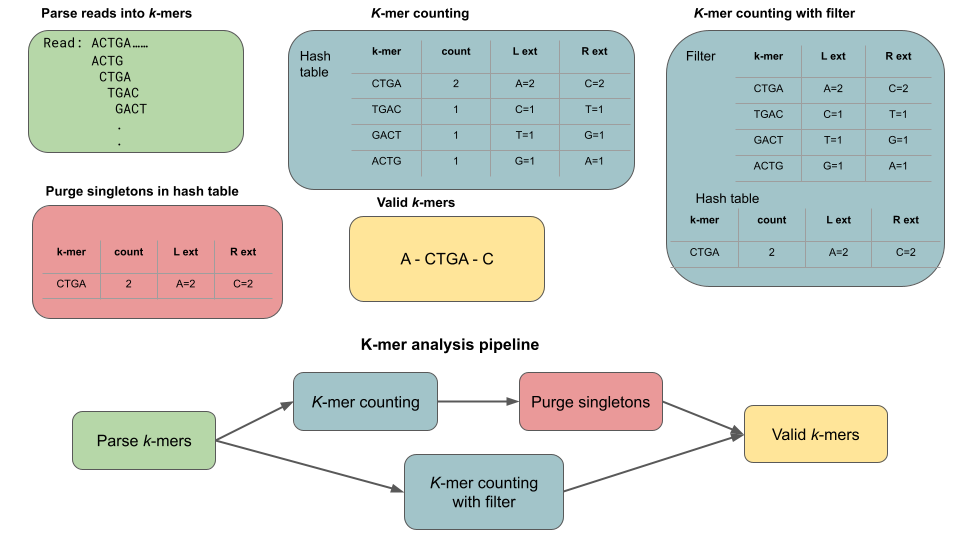
\includegraphics[width=0.9\linewidth]{images/mhm-pipeline.png}
%     \caption{The \textit{k}-mer analysis pipeline in MetaHipMer. A filter can help weed out singleton \kmers from being inserted into the hash table.}
%     \vspace{-0.5em}
%     \label{fig:mhm-kmer}
% \end{wrapfigure}
% \end{figure}

\textbf{Problem definition.}
Metagenome assembly involves reconstructing long contiguous sequences (\emph{contigs}) of genetic material from short input \emph{reads}~\cite{yang2021review}. These reads are strings of bases (the DNA alphabet A, C, G, T) of length 150 to 250 that are produced by gene sequencing machines.
For metagenomes, these reads are extracted from environmental samples (e.g., gut bacteria, or a soil sample) that contain the genes of potentially thousands of microbes, existing at varying abundances.
The reads are error-prone (typically about 0.24\% error per base) and sequencing is done multiple times to ensure every region of genetic material is covered with some error free sequences.

\noindent
\textbf{Importance.}
Metagenomic sequencing provides a culture-independent avenue to investigate the complex microbial communities by constructing metagenome-assembled genomes (MAGs). A MAG represents a microbial genome by a group of sequences from genome assembly with similar characteristics. It enables us to identify novel species and understand their potential functions in a dynamic ecosystem.

\begin{wraptable}{r}{4.5in}
\centering
%\resizebox{\columnwidth}{!}{%
    \begin{tabular}{c c c c c c}
    \toprule
    \textbf{Dataset} & \multicolumn{5}{c}{\textbf{Percentage singleton \kmers}} \\
    \midrule
    & $k=21$ & $k=33$ & $k=55$ & $k=77$ & $k=99$ \\
    \midrule
    WA &  66 & 73 & 76 & 78 & 78  \\
    Rhizo &  67 & 75 & 80 & 83 & 85  \\
    Tymeflies & 63 & 62 & 67 & 69 & 71 \\
    \bottomrule
    \end{tabular}
 %   }
    \caption{Distribution of singleton \kmers in metagenomic data for values of $k$.}
    \label{tab:kmer-dist}
\end{wraptable}

\noindent
\textbf{Challenges.}
Metagenome assembly is challenging due to sequencing error, repetitive content, and library and sequencing bias. In addition, a metagenome sample can contain many thousands of different genomes with varying degrees of similarity, sometimes sharing genetic material, and occurring at vastly different abundances.
%
Furthermore, high-throughput sequencing technology is producing large-amount of metagenomic datasets ranging to TB and PB scales~\cite{hofmeyr2020terabase}. Metagenomic assembly is a complex process consisting of multiple phases and scaling all these phases to terabyte scale comes with a myriad of challenges.

\noindent
\textbf{State of the art.}
MetaHipMer~\cite{GeorganasEHG18,hofmeyr2020terabase} is the first exascale metagenome assembler.
In the approach used by MetaHipMer, the reads are first divided into overlapping substrings of fixed length \emph{k}, called \emph{\kmers}, which are then used to form a de Bruijn graph~\cite{CompeauPeTe11}.
\Kmer counting is the very first step. During \kmer counting, forward and backward extensions of the \kmer and the counts of those extensions are also maintained in the hash table along with the \kmer. Information regarding the extensions and their counts is critical to identifying correct paths in the de Bruijn graph and requires 28 to 52 bytes (depending on $k$) to store each \kmer.
MetaHipmer uses GPUs to speed up the \kmer analysis phase.
In a de Bruijn graph, the vertices are \kmers and edges connect any two \kmers that have an overlap of $k-1$ bases. These vertices are stored in a hash table that is distributed across all the compute nodes in a supercomputer like Perlmutter~\cite{perlmutter} or Summit~\cite{summit}.
Traversal of the de Bruijn graph enables the construction of the contigs (longer sequences).  This approach is more efficient than an all-to-all alignment of the reads, which would be prohibitive for the size of typical metagenome datasets (up to billions of reads).

\noindent
\textbf{Gap and requirements.}
\Kmer counting and analysis is the very first and the most memory-intensive step in the metagenome assembly. The \kmers that occur only once (singletons) are treated as sequencing errors and dropped. In a typical set of metagenome reads, 70--80\% of unique \kmers are singletons, but they still need to be stored and counted in the distributed hash table~\Cref{tab:kmer-dist}.
In the default MetaHipMer implementation, storing the unique \kmers is the most memory-intensive part of the computation and can be roughly an order of magnitude larger than the input data.  The space required to store the \kmers can be much larger than the size of the original raw dataset (up to $10\times$ larger) as \kmers contain a lot of redundant information due to their overlaps.
Weeding out singleton \kmers before inserting them in the hash table to count is critical in any \kmer analysis phase to reduce the memory usage of the counting phase. These singleton \kmers can also be pruned from the hash table after the counting phase. However, that results in the high peak memory usage and much slower running time. MetaHipMer uses filers to weed out singleton \kmers.

The size of the filter and hash table is dependent on the number of unique \kmers. Given that the distribution of \kmers is highly skewed and not known in advance, it is challenging to size the filter and the hash table in order to efficiently utilize the limited memory. Filter and hash tables that can be efficiently resized at runtime will enable efficient memory utilization.


\begin{rproblem}[\textbf{Scale MetaHipMer to petabyte-scale metagenomic datasets on supercomputers}]
Accelerate \kmer analysis phase in MetaHipMer using GPUs and reduce the peak RAM usage to support assembly of petabyte-scale metagenomic datasets from complex biological environments.
\label{rprob:metahipmer}
\end{rproblem}

\section{GPUs and High Performance Computing}

PPoSS targets large-scale systems and we believe that GPUs will form the backbone of future large-scale systems. Why?

With power constraints continuing to be the main bottleneck in increased computing performance, the superior power-performance of GPUs~\cite{Dally:2010:GCT} will make them increasingly attractive at all scales, from mobile devices to laptop and desktop computation to the largest supercomputers. Power constraints are also motivating overprovisioned systems where only a subset of the silicon can be powered at any one time. Such systems tilt toward more heterogeneity, further motivating hybrid systems---and an increased need for GPU-focused computation---as the future norm. We believe accelerators such as GPUs will play a fundamental and integral role in next-generation high-performance computing systems.

Accelerators are becoming increasingly popular in supercomputing, with NVIDIA GPUs programmed with CUDA being a popular  choice for scientific application and infrastucture development.  In the commercial world, the recent and extremely rapid rise of deep-learning  applications~\cite{Amodei:2015:DS2,Chetlur:2014:CEP,Coates:2013:DLW,Hannun:2014:DSU} has led to data-center systems designed for the computationally demanding problem of neural net training, currently dominated by NVIDIA GPUs and CUDA\@.  Nearly every Internet company has NVIDIA-based systems for this purpose.

The most common use of the GPU today is as a coprocessor for compute-intensive tasks. The CPU is responsible for the main runtime, which allocates and populates input data in GPU-accessible memory. The CPU then launches kernels on the GPU to process that memory and fetches the results when the GPU completes its processing. GPUs are certainly prominently featured in some of today's largest distributed memory machines---for instance, ORNL's Titan has an equal number of CPUs and GPUs, but the GPUs account for 90\% of its FLOPS\@. However, the way we program these machines is over 20 years old. We can sum this up in one sentence: GPUs are treated as coprocessors and communicate via MPI where the CPU's runtime is preeminent. This coprocessor model is well-suited for workloads that are large and compute-intensive (to amortize control and transfer overheads) with simple control (to allow the GPU to run without CPU intervention), and is exploited by GPU computing libraries. It is, however, a model where the GPU has little autonomy, and as we will discuss in the next sections, a model poorly suited for our future productive and high-performance computing needs.

We believe the time is right to upend this model and make the GPU more of a first-class processor. We are excited about recent advances in the GPU ecosystem that have added significant functionality enabling our proposed research:

\begin{itemize}
\item Driven by a desire to deliver maximum memory bandwidth, we expect to see both more GPUs on a node (e.g., NVIDIA's DGX2 with 16 GPUs) as well as more GPUs per card. The result is a density that makes using GPUs more attractive and less costly.
\item Inter-GPU and CPU-GPU interconnect is making a significant leap in performance, led by NVIDIA's NVLink (bidirectional 80~GB/s) and OpenCAPI~\cite{DeGelas:2016:OUA}.
\item NVIDIA GPUs now support a unified virtual memory space between CPU and GPU, though manual management is still essential for even single-GPU performance on real-world workloads and certainly for multi-GPU machines. In general, NVIDIA's philosophy has been (1) to expose new hardware mechanisms with functional but limited software support; (2) to see how applications use those mechanisms; and then (3) to optimize their software and  hardware to make those application patterns efficient. Our motivation here is clearly to lead the way in the second step.
\item LLVM now features (open-source) NVIDIA GPU support through Google's gpucc compiler effort~\cite{Wu:2016:GAO}. This work enables compiler research on NVIDIA GPUs that was not previously possible.
\end{itemize}

As GPUs have become an integral part of today's supercomputers, the hardware and software support from vendors and researchers alike has moved beyond the basic model of GPUs communicating only with their host CPU through PCI Express and CPU host memory.

\paragraph{Hardware Support via GPU-to-GPU Communication}
\label{sec:gpudirect}

Historically, all network transfers to or from GPUs had to pass through the CPU and its memory system. This was a significant performance obstacle, particularly due to the inefficiency of copies. Before 2010, a network transfer from a GPU required three copies: (1)~GPU to CPU pinned memory; (2)~CPU copy from user space into driver space; (3)~transfer to the NIC\@. Hardware ``GPUDirect'' support was designed to address this inefficiency. In 2010, the first iteration of GPUDirect shared memory access allowed the sharing of pinned memory between the GPU and the network driver, removing the second copy above. Later GPUDirect advances allowed direct peer-to-peer communication between GPUs on the same PCIe bus (``GPUDirect Peer-to-Peer'', 2011) and direct support for GPU-to-remote-GPU RDMA (``GPUDirect Support for RDMA'', 2012) that does not pass through the CPU at all. NVIDIA offers detailed uidelines~\cite{NVIDIA:2022:DAL} to developers who wish to use this technology.

\paragraph{MPI two-sided and collective support for GPUs}

The predominant access to internode communication has been through MPI, with most work on the two-sided and collective features of MPI\@.  Direct GPU capabilities are part of Cray's MPI and the IBM Platform MPI, but the most significant use has been through MVAPICH2 (since version 1.8) and OpenMPI (also since version 1.8). At a lower level, Mellanox's Infiniband software stack provides direct support for RDMA, and of course Mellanox has now been acquired by NVIDIA (2020) and so we expect this network-GPU tie to only deepen. NVIDIA has implemented a high-performance set of collectives within a single node, which are important as nodes become more powerful and application run multiple MPI ranks per node.  ``NCCL'', NVIDIA's accelerated multi-GPU collective communication library~\cite{Luehr:2016:FMC}, implements broadcast, reduce, all-gather and -reduce, and reduce-scatter for multiple GPUs on a single node.  The ``OSU Micro-Benchmarks'' (version 5.8 as of August 2021)~\cite{MVAPICH:2021:OMB} provide a set of comprehensive benchmarks that include CUDA/OpenACC extensions, primarily latency and bandwidth tests that include MPI collectives.

Ernsting and Kuchen's ``Muesli'' library of algorithmic skeletons~\cite{Ernsting:2012:ASF} was built atop MPI, OpenMP, and CUDA\@. And some MPI packages, such as MVPICH2, take advantage of GPUDirect hardware in accelerating MPI operations. These components are solid building blocks for our work. What they collectively lack is any user-programmable runtimes on the GPU side. We believe the new hardware capabilities and emerging software building blocks strongly motivate the development of user-programmable runtimes to manage and control them.

\section{Why the GPU, and more broadly, massive parallelism?}

The growing difficulty of increasing single-threaded performance~\cite{Ekman:2005:AIL} has motivated a turn to parallelism~\cite{Asanovic:2006:TLO} as the primary means for continuing performance growth in computing. The GPU has emerged as a major player in this landscape. In contrast to a CPU's emphasis on minimizing the latency of a single thread, GPUs instead aim to maximize the throughput of all threads.

\begin{figure}
  \centering
  \begin{tabular}{ccc}
    \includegraphics[width=0.3\textwidth]{figures/deerhound-marked-up} &
    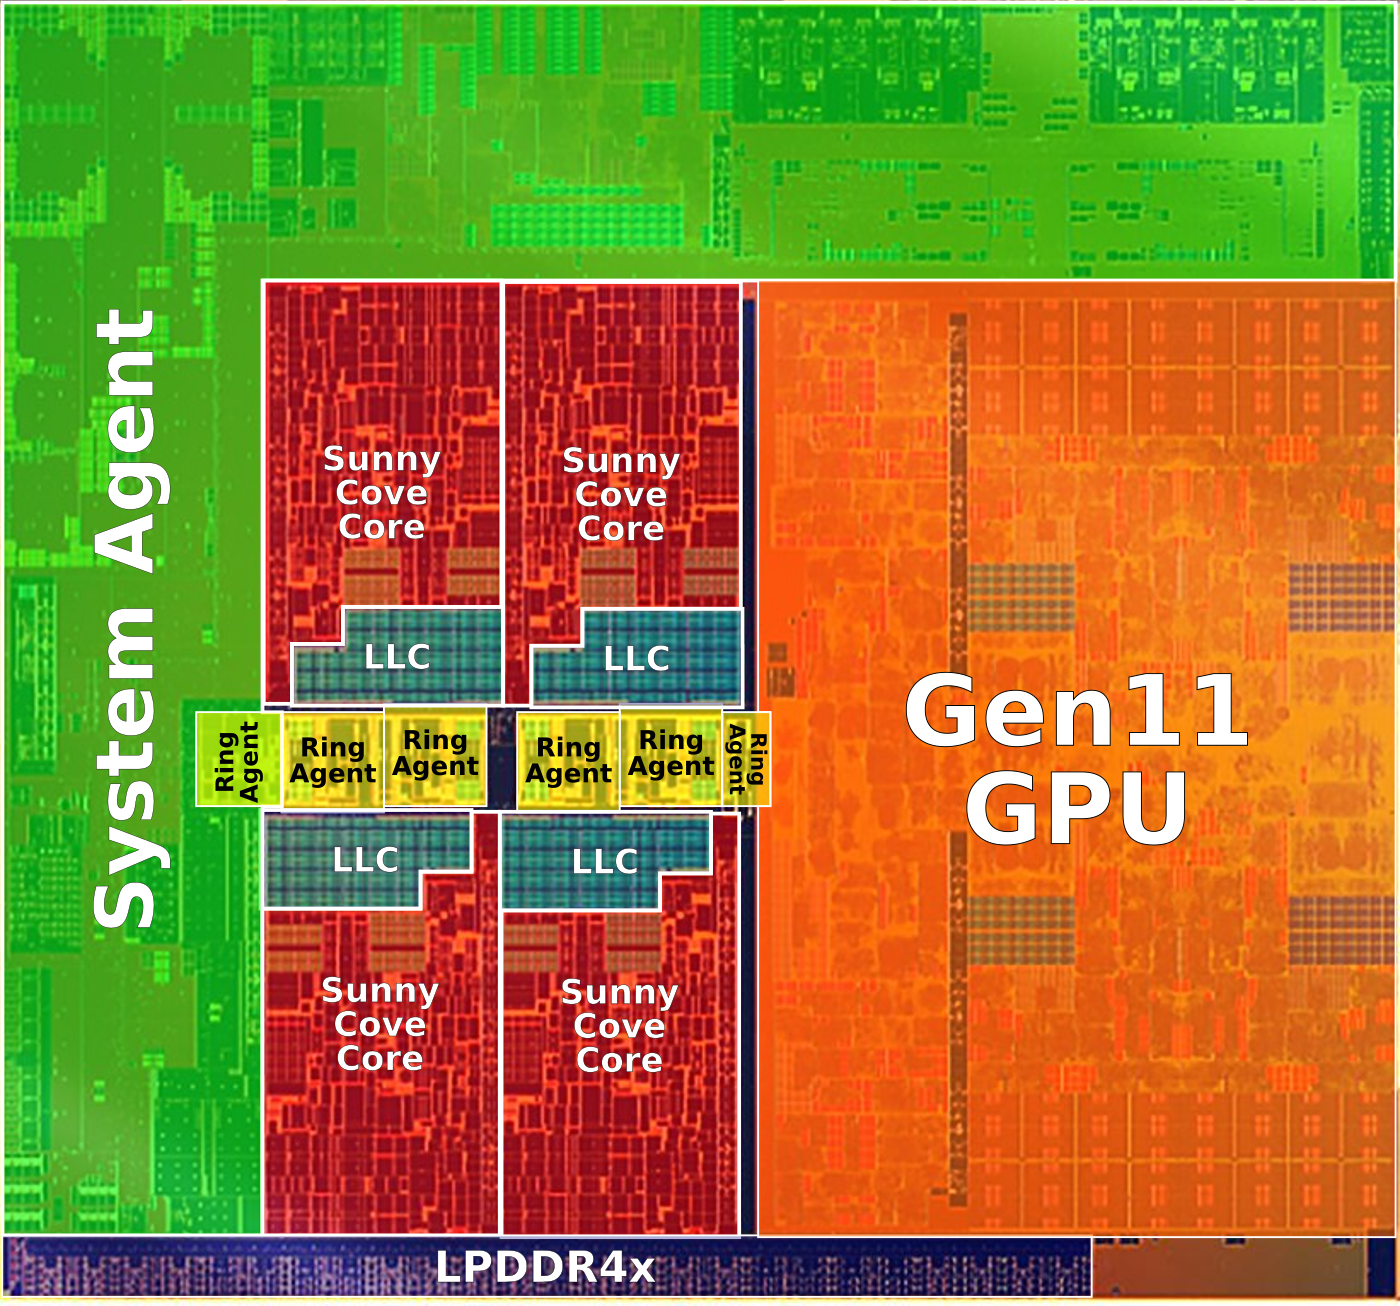
\includegraphics[width=0.3\textwidth]{figures/ice_lake_die_(quad_core)_(annotated)}
  \end{tabular}
  \caption{Over the past fifteen years, the highest-performance computation resources in a mainstream microprocessor have shifted from a small fraction of die area on the CPU to a much larger fraction in an integrated GPU\@. Left: one core of AMD's K8L ``Deerhound'' CPU (2006). Heavy white boxes mark the compute units. Right: Intel Ice Lake hybrid CPU-GPU (2019). Intel's GPU is not only capable of 3D graphics but also general-purpose compute through interfaces like OpenCL\@. \label{fig:gpus-on-modern-processors}} \end{figure}

By focusing on throughput, GPU vendors build designs that are well-suited to address today's most important technology trends. Modern VLSI gives us an increasing number of transistors but little to no increase in clock speeds; GPU vendors have built hardware and software that together scale well with more, rather than faster, hardware resources. The gap (``memory wall'') between processor capability and memory bandwidth continues to grow; throughput-oriented processors like GPUs are designed to amortize increasing memory latency by quickly context-switching to other parallel work. And in a power-constrained world, GPUs have a significant advantage; in his 2010 Supercomputing keynote, Dally cited contemporary figures of 200~pJ/instruction for GPUs and 2~nJ/instruction for CPUs~\cite{Dally:2010:GCT}, with the GPU's power efficiency advantage changing little over the past decade~\cite{Dally:2020:DHA}. It is thus no surprise that even CPU vendors are increasingly emphasizing GPU-like cores on their most recent processors (Figure~\ref{fig:gpus-on-modern-processors}).

With power constraints continuing to be the main bottleneck in increased performance, the superior power-performance of GPUs will make them increasingly attractive. Power constraints are also motivating overprovisioned systems, particularly systems-on-a-chip, where only a subset of the silicon can be powered at any one time~\cite{Esmaeilzadeh:2011:DSA}. Such systems tilt toward more heterogeneity, further motivating hybrid systems---and an increased need for the more energy-efficient GPU-focused computation---as the future norm.
% https://www.nextplatform.com/2022/11/14/testing-the-mettle-of-the-top-supercomputing-iron-on-earth/

But, the front-and-center reason for a continued focus on GPU graph analytics today is outside the scope of graph analytics entirely. The new reality is:

\begin{itemize}
  \item The recent and extremely rapid rise of training deep neural networks for deep-learning applications~\cite{Amodei:2015:DS2,Chetlur:2014:CEP,Coates:2013:DLW,Hannun:2014:DSU}---a field led by NVIDIA GPUs and CUDA---has resulted in NVIDIA-GPU-equipped data centers in nearly every large Internet company and NVIDIA GPUs in each of the three major cloud computing providers. As well, GPUs have made enormous inroads into the largest-scale computations. GPU-centered machines dominate the top of the biannual TOP500 list~\cite{top500:nov2022}, including 7 of the top 10 (\#1 and \#3 have AMD GPUs; 157 total of the 168 GPU-centered machines have NVIDIA GPUs). In systems that have high compute requirements, GPU hardware is now ubiquitous.
  \item Moving data to and from GPUs remains, and appears likely to remain, expensive. Because machine learning and scientific computation are primarily performed today on GPUs, we see an accelerating focus toward ensuring that entire computational pipelines of interest are also on GPUs, to avoid this communication cost. (As an example, it is faster to perform an entire Gunrock breadth-first search on a graph than to transfer that graph between CPU and GPU\@.) So, even if GPU graph applications ran only equally fast as their CPU equivalents, they still offer significant value because they enable faster execution of entire workloads.
\end{itemize}

As a consequence of these two broad trends, NVIDIA has made a large investment into its open-source data science framework, RAPIDS, which has already integrated Gunrock into its codebase and releases, and which will allow us to immediately bring the results from this proposal into widespread use.

%%% Local Variables:
%%% mode: latex
%%% TeX-master: "proposal"
%%% End:


%%% Local Variables:
%%% mode: latex
%%% TeX-master: "main"
%%% End:

%!TEX root =  proposal.tex

\section{Filters}

Filters are a key data structure for compactly representing sets, and they are extensively used in computational biology applications.  The PIs have extensive experience in designing best-in-class filters, both theoretically~\cite{BenderFaGo18,BenderDaFa21,BenderFaKu22b,BenderCoFa23b} and for computational biology~\cite{AlmodaresiPaFe18,PandeyAlBe18,PandeyBeJo18, AlmodaresiPaPa17,PandeyBeJo17b} and for general high-performance computation~\cite{DBLP:conf/usenix/ConwayGCFSTJ20,PandeyBeCo23,PandeyBeJo17a,BenderFaJo12}.
In this section, we articulate the computational challenges in implementing filters in computational-biology applications. 
In particular, filters in HPC settings are compute intensive while being small, making them perfect candidates for GPU implementations.  
However, not all filters have the same functionality, and we will propose algorithm work to create filters than are GPU-friendly, e.g. concurrent, small space, high locality, that will serving the needs of comp. bio. applications.

%==

%Vision of section: different filters have different capabilities. Most famous filter, the Bloom filter, is 

\noindent\textbf{What is a filter?} A \defn{filter} is a data structure for maintaining a set $S\subseteq U$ under approximate membership queries. Specifically, $\texttt{Member}(x)$ returns \textsc{True} if $x\in S$, and returns \textsc{True} with probability at most $\varepsilon$ for $x\notin S$, where $\varepsilon$ is a configurable parameter of the filter.  When a filter returns \textsc{True} erroneously, we say that it has experienced a \defn{false positive}.

A filter is useful because it is small: for $n= |S|$ and $u = |U|$, an error-free dictionary requires $\Omega\left(\log \binom{u}{n}\right) = \Omega(n \log (u/n))$ bits, whereas a filter  takes space at least  lower bound of $\opt + \Omega(n)$ bits~\cite{CarterFG78}.  There are several data structures that meet this lower bound with high probability (w.h.p.), including quotient filters~\cite{Cleary84,PaghPaRa05,DillingerM09,BenderFaJo12,PandeyBJP17,PandeyCDBFJ21}, XOR filters~\cite{GrafLe20} and Ribbon filters~\cite{DillingerW21}.  Bloom filters~\cite{Bloom70} do not meet this lower bound, nor, technically speaking, do cuckoo filters~\cite{FanAnKa14,BreslowJ18}.\footnote{Cuckoo filters are interesting because they do meet the lower bound for reasonable size $n$, but as $n$ grows, the number of bits needed to build a cuckoo filter w.h.p.\ grows to $\Theta(n\log n)$.  In practice, however, cuckoo filters approximate $\opt + \Theta(n)$.}
%
For typical $\varepsilon$, the best filters take one or two bytes per item.

\noindent
\textbf{Filters differ in their functionality, and computational biology software is often limited by the difference in the functionality needed and the functionality of the filter selected.}
Some filters are static, in that they require $S$ to be given at initialization~\cite{GrafLe20,DillingerW21}.  Some filters, such as Bloom filters, allow insertions but no deletions.  Quotient and cuckoo filters are fully dynamic.  Furthermore, quotient filters are \defn{mergeable}, in that two filters can be merged into a single filter, perhaps at the cost of a higher false-positive rate.  Mergeability turns out to be critical in some applications~\cite{conway2020splinterdb,PandeyAlBe18}. Mergeability is closely related to \defn{resizability}.  Any filter can be resized to a larger capacity if we  simply rebuild it from the set $S$.  We refer to a filter as resizable if it can increase its capacity without reference to $S$.  A filter is \defn{incrementally resizable} if we can efficiently resize it by factors of less than 2.  Incremental resizability is a critical to achieving low peak-memory usage in many computational biology applications~\cite{hofmeyr2020terabase,PandeyBJP17,PandeyBeJo17a,MarccaisKi11,wood2014kraken,wood2019improved}, as the size of the set is not known in advance, so existing applications often overprovision the filter size to avoid running out of filter capacity at runtime.

% \mfc{Prashant: why do we need this feature?}  \mfc{We know of no existing filters are incrementally resizable.}



It is possible to turn some filters into \defn{maplets}, which are key-value filters.  That is, each element of $S$ has an associated value.  When querying for an element $x\in S$, one gets the associated value.  And whether $x\in S$ or not, one might get, with small probability, one or more extra values.  Maplets have been shown to be  critical to high-performance key-value stores, as well as \kmer analysis tools to maintain prefix-suffix extensions along with \kmers~\cite{GeorganasEHG18}. 

The PIs Bender, Farach-Colton, Pandey, and Patro used feature-rich filters (including maplets) in bioinformatics systems such as Mantis~\cite{PandeyAlBe18}, Squeakr~\cite{PandeyBeJo18}, deBGR~\cite{PandeyBeJo17b}, Rainbowfish~\cite{AlmodaresiPaPa17}, and MetaHepmer~\cite{mccoy2022high}, MetaHipMer~\cite{McCoyHYP23a} and storage and streaming applications such as SplinterDB~\cite{DBLP:journals/pacmmod/ConwayFJ23} and LERTs~\cite{PandeySiBe20}.
PIs Farach-Colton, Owens, and Pandey implemented high-functionality filters on GPUs~\cite{mccoy2022high, McCoyHYP23a, GeilFO18}. 

To date, all maplets that we know of are based on the quotient filter~\cite{conway2020splinterdb,PandeyBJP17,DBLP:journals/pacmmod/ConwayFJ23}, and we know of no implementation of maplets on the GPU\@.
Our first research problem is:

\begin{rproblem}
Design and build a high-performance maplet for the GPU\@. This will allow us to accelerate ans scale large-scale sequence search and \kmer processing applications using GPUs. 
\end{rproblem}

Building a space-efficient and high-performance maplet is challenging as associating variable-length values with fingerprints results in unaligned memory accesses, which are especially expensive on GPUs. We will develop a quotient filter-based maplet on GPUs as the quotient filters offer compact fingerprint storage and value association. We plan to employ a bulk insertion approach using the sort and merge algorithm to achieve lock-free and high coherence on GPUs. We further plan to explore a two-choice hashing-based vector quotient filter~\cite{PandeyCDBFJ21} and CUDA's cooperative-groups programming model on GPUs to achieve even higher performance.

\begin{rproblem}\label{rprob:resizable-maplet}
Design and build a high-performance incrementally resizable maplet. This will allow us to accelerate and scale large-scale sequence search and \kmer processing applications using GPUs.
\end{rproblem}

The na\"\i{}ve way to resize a maplet is to double its size and move items (perhaps incrementally) from the old filter to the new.  This means that during the transition, which can last quite a long time, both tables must be stored and both tables must be queried. The most direct way to resize a filter is to lock it while we rebuild it at double the size.  We encounter similar problem when resizing hash tables (\S~\ref{sec:hash-tables}), and we will explore the same techniques for resizing filters and hash tables.


We propose to adapt an approach recently proposed by PIs Bender and Farach-Colton: waterfall addressing~\cite{Bender2022}.   Waterfall addressing is a method for addressing into an array (for example for a filter or hash table that uses open addressing) so that the array can grow in small increments.  Each item hashes to a location based on the current size of the array, and when the array resizes, only those items that go into the new piece are moved.  The surprising thing is that this can be done efficiently, but it does require maintaining metadata.  The theoretical version of this result uses pointer-intensive metadata, so this research problem requires developing a new, GPU-friendly metadata scheme and algorithms for distributing the filter. \begin{rproblem}\label{rprob:resizable-maplet-metadata}
Design and build a succinct, GPU-friendly data structure for resizability meta-data.
\end{rproblem}

Finally, some filters, most notably the quotient filter, can be made \defn{adaptive}~\cite{BenderFaGo18}.  A filter is adaptive if its false-positive probability is at most $\varepsilon$ for every $x\notin S$, even if $x$ is repeatedly queried.  In a standard filter, every time $x$ is queried, the filter returns the same answer.  In an adaptive filter, if $x$ is queried and determined to be a false positive, the filter has the option of adjusting itself so that this query is correctly answered as \textsc{False}.  All provably adaptive filters are based on the quotient filter~\cite{BenderFaGo18,Lee21}, although there are some heuristically adaptive filters based on the cuckoo filter~\cite{Mitzenmacher2020}.

\para{Adaptive filters in computational biology}   de Bruijn graphs (dbg) are at the heart of many sequence analysis pipelines~\cite{PandeyBeJo17a,PandeyBeJo17b}. In a (node-centric) de Bruijn graph, each node is a $k$-length subsequence from the underlying biological samples and two nodes are connected via an edge if they share a $(k-1)$-length suffix-prefix overlap.  Traversing long non-branching paths in the de Bruijn graphs, known as unitigs, helps in building long continuous sequences (contigs) as an intermediate step in the assembly process.
% de Bruijn graphs are also used to weed out erroneous sequences in the underlying datasets.
In the graph, each node can have at most four successors by extending the sequence using the four nucleotides (\texttt{A}, \texttt{C}, \texttt{T}, \texttt{G}), and likewise at most four predecessors. Therefore, the set of queries needed to traverse the whole graph is known in advance, and in fact one can think both practically and theoretically about \emph{navigational} representations of such graphs~\cite{Chikhi2015}.
%
de Bruijn graphs are often large enough that they do not fit in main memory. They must also support adding \kmers from new sequences and removing existing \kmers to weed out erroneous sequences.
Therefore, several approaches have been proposed to minimize the space usage of representing a de Bruijn graph by representing it using a  filter~\cite{chikhi2013space}. They can support dbg traversal by querying all four possible extensions from a given node in the filter and building the neighbor list based on positive queries. However, due to false positives there can be some erroneous edges in the graph.
To avoid the false edges, Chikhi and Rizk~\cite{chikhi2013space} proposed to store the de Bruijn graph in a cascading Bloom filter, which is possible because the set of traversal queries is known in advance. Each Bloom filter stores the false positives from querying the earlier Bloom filter using all possible queries during the dbg traversal.

Existing Bloom filter-based solutions are not space-efficient and also do not support deletions. PIs Bender, Patro and Pandey showed how to use quotient filter-based solutions to build a compact representation of de Bruijn and weighted de Bruijn graphs~\cite{PandeyBeJo17b}. However, the quotient filters used in that solution do not adapt during queries and require domain-specific mechanisms and graph invariants to fix approximation errors~\cite{PandeyBeJo17b}.


Dynamic adaptive maplets can be used to build a compact, error-free, and fast representation for de Bruijn graphs. Adaptive maplets can be updated and  would, in theory, take less space than hash tables. Thus, adaptive filters are a good choice for representing and querying de Bruijn graphs, though how they would perform compared to other dynamic succinct de Bruijn graph representations~\cite{DBLP:journals/bioinformatics/AlipanahiKPSB21} remains an open question.



\begin{rproblem}\label{rprob:adaptive-maplet}
Define and prove bounds on adaptive maplets.
\end{rproblem}
The literature on adaptivity has focused on filters.  There are a few possible ways to extend the notion of adaptivity to maplets.  We will explore which of these makes the most sense for our applications and prove bounds on their size and time complexity.
\mab{This will help in applications such as ...}

\begin{rproblem}\label{rprob:dyn-apt-filter}
Design and build a dynamic adaptive maplet to compactly represent de Bruijn graphs.  Compare them to other dynamic succinct de Bruijn graph representations.
\end{rproblem}

In the algorithmic literature on adaptive filters, adaptivity is implemented by varying the number of bits stored in a fingerprint of each item.  When there is a false positive, enough bits are added that the fingerprint of the false-positive query no longer collides with the fingerprint of the item in the set.  Variable-length codes make memory accesses inefficient since the fingerprints are no longer byte-aligned.  We propose to over-adapt by a full byte whenever we have a false positive.  We believe that we can prove that over-adapting in this way does not blow up the space.  Such a scheme will substantially simplify the GPU implementation of adaptive filters.  We believe that all these comments carry over directly to adaptive maplets.


% \textbf{Quotient
% filters}~\cite{Cleary84,PaghPaRa05,DillingerMa09,BenderFaJo12,PandeyBJP17,pandeySigmod21}
% represent a set approximately by compactly storing small fingerprints of the
% items in the set via Robin Hood hashing~\cite{CelisLaMu85}. The quotient filter
% uses $1.053 (2.125 + \log_21/\epsilon)$ bits per element, which is less than the
% Bloom filter whenever $\epsilon \leq 1/64$, which is the case in almost all
% applications. It supports insertion, deletion, lookups, resizing, and merging.
% The counting quotient filter (CQF)~\cite{PandeyBJP17}, improves upon the
% performance of the quotient filter and adds variable-sized counters to count
% items using asymptotically optimal space, even in large and skewed datasets. In
% the counting quotient filter, we can also associate small values with items
% either by re-purposing the variable-sized counters~\cite{PandeyABFJP18Cell} to
% store values or by explicitly storing small values with the remainders in the
% table~\cite{PandeySMB20}.



% \textbf{Two-Choice filters}~\cite{pandeySigmod21} organize fingerprints
% compactly in blocks similar to the cuckoo filter. However, unlike the cuckoo
% filter, there is no kicking. The blocks in the two-choice filter are larger in
% size ($\approx \log{n}$, where $n$ is the number of items which is usually the
% size of the cache line on most machines) than the cuckoo filter and
% power-of-two-choice hashing is used to reduce the variance across the blocks and
% achieve a high load factor. During insertions if both blocks corresponding to a
% fingerprint are full then the data structure is declared full. The
% power-of-two-choice hashing enables the filter to probe exactly two cache lines
% during inserts and queries and write to a single cache line during inserts.
% Given the larger block sizes the vector quotient filter~\cite{pandeySigmod21}
% uses quotienting (similar to the quotient filter) to organize fingerprints
% inside blocks. It divides the fingerprints into a quotient and remainder part
% and only stores the remainder in the slot given by the quotient. It uses two
% additional metadata bits to resolve collisions among quotients.

\iffalse

\subsection{Analysis of filter designs}

We now look at the dynamic filters discussed in~\Cref{sec:prelim} and evaluate
them based on the GPU design principles.  Our goal is to identify the filters
that offer necessary features such as deletions, counting, and value
associations and at the same time satisfy most of the design principles.  We
will further discuss the challenges of implementing these filter on the GPUs to
achieve high speed operations.

Bloom filters are easy to implement on the GPU as they only require test and set
operations. These operations can be implemented using atomic operations and
achieve low thread divergence. However, each operation results in multiple cache
misses and therefore Bloom filters have low memory coherence. They also have
sub-optimal space usage. Moreover, Bloom filters do not support deletions,
counting\footnote{The counting Bloom filter~\cite{FanCaAl00}, a variant of the
Bloom filter, supports counting but it comes at a high space-overhead which
makes it highly inefficient in practice.}, and associating small values with
items.
% that many data analytics applications require.

Blocked Bloom filters are better suited to GPUs.  Each operation requires
probing inside a single block. They achieve low thread divergence, high memory
coherence, a high degree of parallelism, and atomic operations. Thus, blocked
Bloom filters can satisfy all the GPU design principles. However, blocked Bloom
filters have a high false-positive rate compared to Bloom filters and also do
not support necessary features like deletions and counting.

Operations in the quotient filter have high cache locality which makes it an
appropriate choice to achieve high memory coherence. However, insert operations
in the quotient filter requires shifting fingerprints which makes it harder to
use atomic operations and also results in high thread divergence. However, the
quotient filter can support all the necessary features like deletions, counting,
and associating small values with items which makes the quotient filter a highly
usable data structure that multiple applications can benefit from.

It is quite challenging to achieve high speed operations while maintaining all
of the features in a GPU implementation of the quotient filter. Geil et
al.~\cite{Geil:2018:QFA} implemented a preliminary version of the GPU quotient filter.
However, that implementation was adapted from Bender et al.'s quotient
filter~\cite{BenderFaJo12}, which did not have all the features, like counting
and value association, and also had higher space overhead. Furthermore, Geil et
al.'s GPU-based quotient filter has implementation-specific limitations (e.g., it
supports a fixed false-positive rate and can only be sized to store less than
$2^{26}$ items) resulting in poor performance and limited scalability.

The cuckoo filter stores fingerprints in fixed size blocks. This design is
amenable to high memory coherence and low thread divergence. Atomic operations
can also be used to read and write fingerprints. However, the cascading sequence
of reads and writes to random memory locations makes the cuckoo filter hard to
implement efficiently on the GPU\@. In particular, at high load factors when the
number of kicked items becomes high, each insertion will result in very low
memory coherence. Moreover, each kicking operation results in multiple
cache-line writes. This makes it challenging to achieve high speed operations in
a GPU cuckoo filter. Moreover, cuckoo filters do not support counting and
associating small values with items.

The two-choice filter has the advantages of the cuckoo filter design. It has
fixed size blocks. Each operation requires probing into exactly two blocks, and
inserts and deletes only write into a single block. This results in low thread
divergence, high memory coherence, and a high degree of parallelism. However,
due to large block sizes a more sophisticated structure is required to maintain
fingerprints inside each block. Therefore, it is not straightforward to use
atomic operations to read or write fingerprints inside blocks. It is a
challenging task to implement a two choice filter on the GPU using atomic
operations to achieve high throughput.

\fi

\section{Sketches}



The challenge of computing properties of massive data streams in limited space has inspired a deep and beautiful literature on streaming algorithms and database systems. In the dynamic streaming model, the input is defined by a sequence of items of length $N$ and only $O(\polylog N)$ {RAM} is available for computation. For most interesting graph problems, such as matchings or spanning forests, this is not enough space to even represent a solution. Algorithms for these problems instead use the dynamic semi-streaming model~\cite{insertonlysemistreaming}, which allows more space (specifically, $O(n \; \polylog n)$ \acro{RAM} is available for a graph of $n$ nodes and $m$ edges). Note that this is still not enough space to store the graph explicitly, unless the graph is sparse: any lossless representation requires $\Omega(m))$ space, which can be $\Omega(n^2)$ for the densest graphs. In this model, the input graph is defined by a stream of edge insertions and deletions, and this stream is delivered to the algorithm a small number of times (typically once).

Semi-streaming algorithms have several advantages that, in theory, make them powerful tools for computing on graphs at scale.  Since these algorithms require an up to $\Theta(n)$-factor less space than an explicit representation of a dense graph, they are able to process much larger graphs given a fixed amount of memory. Effectively, all dynamic semi-streaming algorithms are equivalent to linear sketching algorithms~\cite{li2014sketchuniversal}, which are highly parallelizable, easy to distribute, robust to arbitrarily ordered input streams, and have good data locality. In a nutshell, they trade more computation for a smaller space requirement. %\jdo{Is the previous sentence correct?}
The benefits of practical implementations of semi-streaming algorithms would be significant, vastly increasing the scale of graphs which can be processed even when these graphs are too large for fast memory, change over time, or even are generated in real time (for example, from sensors measuring large-scale real-world phenomena, or from dynamic connections or interactions in a large network).

While many dynamic semi-streaming graph algorithms\cite{Ahn2012, AhnGM12b, AhnGM13, GuhaMT15, KapralovLMMS13, ChitnisCEHMMV16, AssadiKL16, McGregorVV16, pagh2012colorful, 10.1007/978-3-662-48054-0_39, clustering, 10.1007/978-3-319-21398-9_57, streamsetbounds, Chakrabarti2015IncidenceGA, kveton2016graphical, CrouchMS13} are known in the theory literature, prior to our Sept.\ 2021 prototype~\cite{graphzeppelin}, there were \emph{no} implementations of these algorithms in use in academia or industry.  One of the primary bottlenecks of these algorithms is the high computational cost of their linear sketching subroutines. This difficulty leads us to the GPU.

\prashant{Add comp bio work in minhash for Jaccard similarity, edit distance, HyperlogLog.}


\begin{rproblem}
Can we develop algorithms that can replace hashing with batch sorting.
\end{rproblem}

\prashant{Efficient sketching on GPUs.}

% \prashant{Notes for Martin.}

% \prashant{Given a fastq file containing raw sequencing reads. Can we quickly and space-efficiently (maybe sublinear time and space?) estimate a frequency distribution for \kmers for a given $k$?
% Specifically, we are interested in estimating the total number of \kmers, the total number of distinct \kmers, the total number of \kmers with a given count C?}

\begin{rproblem}
Develop data structures for indexing and searching low-dimensional embeddings (based on minhash) for raw genomic and metagenomic data.
\end{rproblem}


\begin{rproblem}
Build a GPU-enabled cardinality estimator for \kmers in raw sequencing samples (genomic, transcriptomic, metageomic).
\end{rproblem}

% best distinct elements count sketch AFAIK: https://people.eecs.berkeley.edu/~minilek/publications/papers/f0.pdf this has likely been implemented, but i haven't verified. I will check if i have time. and for fun, a differentially private solution to the problem (which i have not read): https://arxiv.org/abs/2001.11932


\begin{rproblem}
Develop algorithms that are close to communication lower bound to compute the similarity score for two set of \kmers in a distributed setting.
\end{rproblem}



\begin{rproblem}
Design and build a system to compute similarity score (Jaccard index) for \kmer sets in a distributed-setting.
\end{rproblem}


% i am not super familiar with the work on sketching set similarity but this paper seems promising: https://www.itu.dk/people/pagh/papers/oddsketch.pdf there is also this implementation-focused paper that includes another sketch to solve the problem and mentions the prior paper: https://dl.acm.org/doi/abs/10.1145/3292500.3330825

\section{Hash tables}
\label{sec:hash-tables}

% \prashant{Notes for Martin/John.}

% \prashant{Scale up: We need hash tables with: fine-grained resizing on GPUs. Applications often do not know the number of items in advance. If they under size the hash table they fail at run time and if they oversize they waste memory.}

% \prashant{Scale out: We need hash table that can be distributed across multiple nodes in HPC clusters. However, when partitioning data across multiple nodes there are two challenges: First, we need to reduce the load variance across nodes. Second, we need to reduce the communication volume to while constructing the hash table and also to perform operations on the hash table. Operations can include: performing a join/intersection across two distributed hash tables.}

% \prashant{Forward and backward extensions of the \kmer and the counts of those
% extensions are also maintained in the hash table along with the \kmer.
% Information regarding the extensions and their counts is critical to identifying
% correct paths in the de Bruijn graph and requires 28 to 52 bytes (depending on
% $k$) to store each \kmer.}

% \prashant{HT is built for multiple values of $k$ across different iterations of the contig mapping. The HT is required to support variable-length keys ranging from 32-bits to 200 bits.}


% \prashant{HT use case in MetaHipMer}

% \prashant{In the approach used by MetaHipMer, the reads are first divided into overlapping substrings of fixed length-$k$, called \kmers, which are then used
% to form a de Bruijn graph. In a de Bruijn graph, the
% vertices are \kmers and edges connect any two \kmers that have an overlap of
% $k-1$ bases. These vertices are stored in a hash table that is distributed
% across all the compute processes.  The size of the hash table is dependent on
% the number of unique \kmers which is not known in advance. Currently, an approximation of the number of unique \kmers is used to size the HT. If it is an over approximation GPU device memory is wasted and if it is an under approximation then \kmers are arbitrarily dropped when HT becomes full resulting in dropped quality of the final result.}

% \john{I don't see any requirement here for stability. In fact I think stability is probably not what we want because we probably want to periodically load-balance, or at least explore the cost vs.\ benefit of load balancing as part of our work. So I don't think any stability stuff gets included.}

% \prashant{I think we need stability for local, single-GPU hash tables. With stability we can avoid data movement and hence less contention. So, stability is important to achieve high concurrency. For the distributed setup, yes, we need to move items for load balancing.}

% \john{Question for Prashant. Do we need to support deletes? If so we probably want to have a garbage collection effort.}

% \prashant{Yes, we need deletes. Garbage collection could be an efficiency way to support deletes. We can enter tombstones during deletes and garbage collect in a lazy manner. Important to achieve high concurrency.}

% \john{Here's the stuff I want to write up. (1) Build dynamic hash tables with variable-length keys. I don't know how to do that but I know it's not really been done on GPUs. One possibility: Hash the \kmers and use the hash as the key into the hash table. Of course we can also look to natively support variable-sized keys. (2) Overlapping communication and on-GPU-hash-table operations, so we don't have periods with all-compute-no-communicate and all-communicate-no-compute. (3) Explore tradeoff between better load balance and cost of load balance. (4) Explore tradeoff between more locality and reduced hash table efficiency (this is basically ``can we reduce overall communication by trying to keep/move hash table entries to their home nodes, and does that help overall performance''). (5) Communication management, in particular bundling up small communications into larger ones to achieve better bandwidth.}

% \prashant{All these points are great. Just to add one point.. we can say we will use locality-sensitive hashing and domain knowledge to smartly partition data to reduce communication volume.}

% \noindent\john{\hrulefill{}}

While building static single-GPU fixed-key-size hash tables can be done efficiently and with high load factors~\cite{Awad:2023:AAI}, scaling and improving the functionality of GPU hash tables to support the bioinformatics workloads in this proposal presents several significant research challenges. In particular, we must address three important and orthogonal problems:

\begin{rproblem}
  Supporting more functional \textbf{dynamic} hash tables that can incrementally add and delete keys and values
  \label{rprob:dynamic-gpu-hashtable}
\end{rproblem}

\begin{rproblem}
  Extending hash-table support for \textbf{variable-length keys}
  \label{rprob:variable-hashtable}
\end{rproblem}

\begin{rproblem}
  \textbf{Distributing these hash tables across multiple GPUs} for both increased capacity and increased performance
  \label{rprob:dist-hashtable}
\end{rproblem}

\subsection{Dynamic hash tables}

While a large body of research has addressed building and querying static GPU hash tables, work on dynamic GPU hash tables~\cite{Ashkiani:2018:ADH,Junger:2020:WAL,Li:2021:DDH,Zhou:2021:DAD} has been much less common. This previous work has shown the possibility of low-level data structures for supporting dynamic operations (our work~\cite{Ashkiani:2018:ADH} uses buckets of linked lists, each made of warp-wide slabs, as its fundamental atom) but this work is generally balanced (and achieves high performance) only when its bucket count and average bucket size are near-optimal. For some applications this may be acceptable. For the bioinformatics applications we target, we expect the amount of stored data in a hash table (e.g., \kmer storage) to vary widely over the runtime of one application, and existing methods are likely to perform poorly. In the CPU world, such rebuilding is common, and handled in the background, but no such runtime capability is available in the GPU world. As well, existing work does not automatically reclaim memory on deletes, which is important in applications (such as \kmer analysis) that feature both insertions and deletes.

\paragraph{Proposed approach}

We propose to address these deficiencies (rebuilding for optimal sizing and reclaiming memory) by leveraging NVIDIA's MPS (``MultiProcessing Service'') capability to simultaneously run two applications. One application, and the one that will take most GPU resources, will be the hash table and its umbrella application. The second will be a small ``runtime'' application that uses modest resources and will rebuild and reclaim memory alongside the main application. This can be done without programmer intervention, without stopping the entire application to rebuild the data structure or reclaim memory, and most importantly, can reduce register usage for the main application by offloading its operations into the runtime and thus improve aggregate performance.

\subsection{Variable-length keys}

\Kmer analysis requires the storage of \kmer keys of variable length (32--200 bits). Existing dynamic hash tables only handle fixed-length, word-sized keys. Fortunately, the size of these keys is bounded, and this aids our proposed solution.

\noindent
{\bf Proposed approach.}
We anticipate two directions of research that will allow us to provide the necessary support:

\begin{itemize}[noitemsep,nolistsep,leftmargin=*]
  \item The GPU's high computational capability likely makes it tractable to perform a large number of arithmetic operations on each key (as we noted in our 2011 static-hash-table work~\cite{Alcantara:2011:BAE}, ``we can run up to 1000 instructions per memory update and remain memory bound''). Thus we will investigate computing a hash function (e.g., MD5) on each key and use the (fixed-size) hash value as the key. If necessary, we can also store the keys themselves: modern GPU memory managers (e.g., Ouroboros~\cite{Winter:2020:OVQ}) maintain multiple pools of memory, each of which satisfies requests of different sizes. Again because of the bounded size of \kmers, we believe we can specialize a memory manager to only a few pools and yet still maintain high memory load factors.
  \item We also will study the design of a cascade of hash tables, where keys in the first hash table are the first 32 or 64 bits of the \kmer and the value associated with each key is a second hash table, whose keys represent the next 32 or 64 bits, and so on. This strategy would be impractical for arbitrary-length keys but for \kmers, with their bounded lengths, it appears to be feasible.
\end{itemize}

\subsection{Distributed hash tables}

GPU memory is modest in size and to scale up, rather than pay the high communication cost of communicating between CPUs and GPUs through the slow PCIe bus, the most common approach is to scale \emph{across} GPUs using faster technologies like NVLink and Infiniband. However, naively partitioning the hash table across GPUs and performing fine-grained, synchronous access to it is unlikely to permit competitive performance.

\noindent
{\bf Proposed approach.}
Thus we propose several directions that can help mitigate the potential performance issues of partitioning. First, we will build our application in a chunked and pipelined way so that we can simultaneously compute hash table keys for chunk $n+2$, use inter-GPU communication to be fetching values for chunk $n+1$, and process the results for chunk $n$. Such an approach is necessary to best use our computation and communication resources. Second, we will need to bundle up small-grained communications into larger packets and only send those packets when they are full to best use the full bandwidth of the communication resources. Finally, we will investigate distributed hash table strategies that allow us to trade off (i) better load-balance vs.\ the cost of that load balance and (ii) better locality vs.\ the penalty in hash table efficiency (for instance, locality-sensitive hashing techniques and domain-specific knowledge to place pieces of the hash table where they will most frequently be used).    Essentially, a random partition will give us excellent load balance and efficiency, but will result in a maximal amount of communication. We propose to relax (rather, explore the consequence of relaxing) ideal load balance and ideal efficiency to reduce overall communication volume.


% \noindent\john{\hrulefill{}
% I don't find anything under here relevant.
% \noindent\hrulefill}

% Hash tables are a core data structure in many applications, including key-value
% stores, databases, and big-data-analysis engines, and are included in most
% standard libraries.  Hash-table performance can be a substantial bottleneck for
% many applications~\cite{NealZu21,FanAn13,MetreveliZe12}.


% We argue that two stricter criteria, \emph{referential stability} and \emph{low
% associativity} should be optimized to yield high performance on PMEM.  As we
% will see, these two goals seem to be at odds with each other, and part of the
% innovation  of our hash table design is that it simultaneously achieves both.
% Naturally, the third design goal for a high-performance hash table is
% \emph{compactness}, but compactness also seems at odds with referential
% stability and low associativity.

% A hash table is said to be \defn{stable} if the position where an element is
% stored is guaranteed not to change until either the element is deleted or the
% table is resized~\cite{sandersstability,originalstability,KnuthVol3}.
% Stability offers a number of desirable properties.  For example, stability
% enables simpler concurrency-control mechanisms and thus reduces the performance
% impact of locking.  Moreover, since elements are not moved, writing is
% minimized, which improves PMEM performance.
% expensive than reads~\cite{pmem-measurements}.

% The \defn{associativity} of a hash table is the number of locations where an
% element is allowed to be stored.\footnote{Associativity is often associated with
% caches that restrict the locations an item may be stored in.  Here we refer to
% \emph{data structural associativity}, which is a restriction on how many
% locations a data structure may choose from to put an item in, even on fully
% associative hardware.} The best known low-associative (DRAM) hash table is the
% cuckoo hash table~\cite{Pagh:CuckooHash,PaghRo01}.  In the original design, each
% element has exactly two locations in the table where it is allowed to be stored,
% meaning that the associativity is two.  Low associativity yields a different set
% of desirable properties---most importantly, it helps search costs. For example,
% searching for an element in a cuckoo hash table is fast because there are only
% two locations in the table to check.  In addition, low associativity can enable
% us to further improve query performance by keeping a small amount of metadata~\cite{pandey2022iceberght}.


% In combination, stability can be used to achieve high insertion throughput in
% PMEM, where writes are expensive, and low associativity can be use to achieve
% high query  performance.  Furthermore, we also show how stability enables
% locking and concurrency-control mechanisms to be simplified, leading to better
% multithreaded scaling and simpler designs for crash consistency.

% Unfortunately, there is a tension between stability and low associativity.  If a
% hash table has associativity $\alpha$, and elements cannot move once they are
% inserted, then an unlucky choice of $\alpha$ locations for $\alpha$ elements can
% block a $(\alpha+1)$st element from being inserted.  As $\alpha$ decreases, the
% probability of such an unlucky event increases.  Cuckoo hashing reduces the
% probability of these bad events by giving up stability via \defn{kickout
% chains}, which are chains of elements that displace each other from one location
% to another. Practical implementations~\cite{LiAn14} generally increase the
% number of elements that can be stored in a given location---and thus the
% associativity---to reduce the kickout-chain length and increase the
% maximum-allowed \defn{load factor}, i.e, the ratio of the total number of keys
% in the table to the overall capacity of the table.


% Similarly, there is a three-way tension between space efficiency, associativity,
% and stability.  For example, cuckoo hash tables can be made stable if they are
% overprovisioned so much that the kickout-chain length reaches 0.  Such
% overprovisioning directly decreases space efficiency, but it also increases
% associativity.  Linear probing hash tables are stable (assuming they use
% tombstones to implement delete) but, as the load factor approaches 1, the
% average probe length for queries goes up, increasing associativity.  Other
% open-addressing hash tables have a similar space/associativity trade-off.
% Chaining hash tables are stable, but they have large associativity and
% significant space overheads.  CLHT~\cite{david2015asynchronized} improves query
% performance despite high associativity by storing multiple items in each node,
% but this further reduces space efficiency.

% \iffalse
% \subsection{B-trees}

% The \btree(or B$^+$-tree\footnote{A \bplustree is a scan-optimized variant of
% \btrees that stores all data records in the leaves and only pivot keys in the
% internal nodes. The \bplustree is the widely implemented variant of the \btree
% in real-world applications as it supports faster range
% scans~\cite{mongodb,couchdb,scylladb,conway2020splinterdb,postgresql}. In this
% paper, we refer to \bplustree as the \btree.})~\cite{BayerMc72} has been the
% fundamental access path structure in databases and storage systems for over five
% decades~\cite{Comer79,graefe2010survey}. \btrees are an extension of
% self-balancing binary search trees to arbitrary fanouts (with more than two
% children per node). They store elements in each node in a sorted array.  Given a
% cache-line size $Z$~\cite{AggarwalVi88}, a \btree with $N$ elements and node
% size $B = \Theta(Z)$ supports the point operations \proc{insert} and \proc{find}
% in $O(\log_B(N))$ cache-line transfers in the I/O model~\cite{AggarwalVi88}.
% \btrees are one of the top choices for in-memory indexing~\cite{ZhangChOo15} due
% to their cache efficiency though they were initially introduced for indexing
% data stored on disk~\cite{BayerMc72}. In this paper, we study and improve the
% performance of in-memory \btrees.

% \btrees are especially popular in databases and file systems because they
% support logarithmic point operations (inserts and finds) and efficient range
% operations (range queries and scans) that read blocks of
% data~\cite{Knuth98,rodeh2013btrfs}.  They are also extensively used as the
% in-memory index in many popular databases such as MongoDB~\cite{mongodb},
% CouchDB~\cite{couchdb}, ScyllaDB~\cite{scylladb}, PostgreSQL~\cite{postgresql},
% and SplinterDB~\cite{conway2020splinterdb}.
% \fi

\section{String data structures}

%
String pattern matching is one of the most common and most computationally intensive problem in computational biology.
%
String pattern matching is the problem of counting or locating occurrences of a query text pattern $P$ within a large database text $T$. While not limited to the analysis of biological sequences, string pattern matching is integral to many tasks in computational biology, including mapping sequence reads to a reference genome~\cite{li2009fast,langmead2009ultrafast}, sequence to graph alignment~\cite{Jain2020}, taxonomic classification~\cite{menzel2016fast,kim2016centrifuge}, sequencing error correction~\cite{huang2017efficient}, and seeding for sequence alignments~\cite{buchfink2015fast,altschul1990basic,steinegger2017mmseqs2}.

The need for high-throughput pattern matching in computational biology has motivated numerous approaches including hashing, lookup tables, suffix arrays~\cite{manber1993suffix}, and compressed suffix array data structures such as the FM-index~\cite{ferragina2000opportunistic}.
FM-index is based on Burrows-Wheeler transform~\cite{burrows1994block}. The Burrows-Wheeler transform (BWT) is a reversible text transform that was originally proposed for lossless data compression.

% Strings and subsequences appear in a plethora of computational biology problems because the basic types of DNA, RNA, and protein molecules can be represented as strings—pieces over a given alphabet of DNA as strings over the alphabet {A,C, G, T } (representing the four bases adenine, cytosine, guanine, and thymine, respectively), pieces of RNA as strings over the alphabet {A,C, G, U} (with uracil replacing thymine) and proteins as strings over an alphabet of 20, corresponding to the 20 amino acid residues.

% Let $A$ be a finite alphabet consisting of a set of characters (or symbols).  The cardinality of the alphabet denoted by $|A|$ expresses the number of distinct characters in the alphabet.  A string or word is an ordered list of zero or more characters drawn from the alphabet. A word or string $w$ of length $n$ is represented by $w[1 \ldots n] = w[1],w[2], \ldots ,w[n]$, where $w[i] \in A \; for \; 1 \leq i \leq n$ and $|w|$ denotes the length of $w$. The empty word is the empty sequence (of zero length) and is denoted by $\phi$.  A list of characters of $w$, appearing in consecutive positions, is called a \emph{substring} of $w$, denoted by $w[i \ldots j]$, where $i$ and $j$ are the starting and ending positions, respectively. If the substring starts at position 1, then it is called a \emph{prefix}, whereas if it ends at position $n$, then it is called a \emph{suffix} of $w$. However, an ordered list of characters of $w$ that are not necessarily consecutive is called a \emph{subsequence} of $w$.

Use of the FM-index across applications is due to its fast performance and low memory footprint. Unfortunately, its adoption is likely limited by the lack of an optimized and lightweight FM-index library; the only robust, currently maintained FM-index implementations are SeqAn3 library~\cite{Reinert2017} and AWFM-index~\cite{Anderson2021}.
%
Furthermore, FM-index is a static data structure. It saves space at the cost of updatability. However, sequences are often added and deleted in computational biology datasets and existing applications have to rebuild the string indexes from scratch to support updatability.
%
Finally, constructing compressed string indexes like BWT and FM-index is memory intensive. Existing tools like BOSS~\cite{Bowe2012} and VARI~\cite{Muggli2019} use disks to mitigate the high memory requirements to construct string index. They need to write out the intermediate results to disk and page them back and forth. This results in suboptimal construction speed.

\begin{rproblem}
Prove a lower-bound for space and run time to support updates in FM-index.
\end{rproblem}


\begin{rproblem}
Prove lower bounds for space and run time for sequence to graph alignment.
\end{rproblem}

\begin{rproblem}
Design and build a sequence to graph alignment library for GPUs.
\end{rproblem}


\begin{rproblem}
Design and build a sequence to graph alignment library for GPUs in distributed-memory when the sequence graph is stored across multiple GPUs.
\end{rproblem}

% \section{Cross-cutting Concerns}
\section{Evaluation plan}

% The Project Description must contain a section titled "Evaluation Plan" that (a) includes a timeline of proof-of-concept implementations of the key components; and (b) outlines how the project's success will be measured.

\subsection{Timeline}

\begin{description}
\item [Year 1:] Develop theoretical models for GPU-based data structures. Build initial prototypes of filters, hash tables, sketches, and string data structures for single-node GPUs.

\item [Year 2:] Explore computational biology applications such as taxonomic classification for metagenomic data, raw sequence search, and pangenomics to develop a common data structure API. Build single-node GPU-enabled software tools for common data processing pipelines such as k-mer analysis and sequence alignment.

\item [Year 3:] Develop a single-node GPU-based compact and dynamic data structure library. Integrate the data structure library in computational biology tools.

\item [Year 4:] Develop models for multi-node multi-GPU data structures for computational biology problems. Build prototype multi-node multi-GPU data structures.

\item [Year 5:] Scale out computational biology applications in HPC environments such as Perlmutter and Summit supercomputers using multi-node multi-GPU data structures library and perform petabyte scale data analyses.
\end{description}

\begin{ganttchart}[
  x unit=0.6cm,
  vgrid,
  hgrid,
  y unit title=0.4cm,
  title height=1,
  y unit chart=0.4cm,
  bar height=0.6,
  ]{1}{20}
  \gantttitle{2023}{1}
  \gantttitle{2024}{4}
  \gantttitle{2025}{4}
  \gantttitle{2026}{4}
  \gantttitle{2027}{4}
  \gantttitle{2028}{3}\\
  %%%%%%%%%%%%%%%%%%%%%%%%%%%%
  \ganttgroup{Algorithms}{1}{20}\\
  \ganttbar{Task 7}{1}{3}\\
  \ganttbar{Task 8}{4}{7}\\
  \ganttbar{Task 9}{7}{10}\\
  \ganttbar{Task 11}{11}{14}\\
  \ganttbar{Task 17}{4}{7}\\
  %%%%%%%%%%%%%%%%%%%%%%%%%%%%
  \ganttgroup{Systems}{1}{20}\\
  \ganttbar{Task 5}{1}{3}\\
  \ganttbar{Task 6}{3}{5}\\
  \ganttbar{Task 10}{6}{9}\\
  \ganttbar{Task 13}{10}{2}\\
  \ganttbar{Task 14}{3}{6}\\
  \ganttbar{Task 15}{7}{10}\\
  \ganttbar{Task 18}{8}{12}\\
  \ganttbar{Task 19}{13}{16}\\
  %%%%%%%%%%%%%%%%%%%%%%%%%%%%
  \ganttgroup{HPC}{1}{20}\\  
  \ganttbar{Task 12}{11}{14}\\
  \ganttbar{Task 16}{13}{16}\\
  \ganttbar{Task 20}{17}{20}\\
  %%%%%%%%%%%%%%%%%%%%%%%%%%%%
  \ganttgroup{Applications}{1}{20}\\  
  \ganttbar{Task 1}{3}{16}\\
  \ganttbar{Task 2}{5}{18}\\
  \ganttbar{Task 3}{2}{20}\\
  \ganttbar{Task 4}{3}{20}
\end{ganttchart}

\subsection{Measuring Success} We will combine our systems and theory advances into a standalone GPU library for compact, dynamic, and distributed data structures that we will link with our focus computational biology applications. We expect to be measured on the success of these the data-structure library and these applications.

\noindent
\paragraph{Success for our data-structure library}

\label{sec:sw-methodology}

\begin{itemize}[noitemsep]
  \item Our library is the data-structure substrate for the three computational biology applications described below, for both single-GPU and multi-GPU/multi-node configurations.
  \item Our library embodies best practices in software development: open-source software with an Apache 2.0 license, available via Github; a suite of functional and performance tests; a benchmarking suite to evaluate the performance of these data structures and help drive subsequent modules; use of code-coverage tools together with these tests; use of continuous-integration and continuous-development tools and methodologies; internally documented code with Doxygen; and high-level developer documentation that guides use of the library. Particularly with our widely cited and used Gunrock library~\cite{Wang:2017:GGG} for GPU graph analytics, we have extensive experience with building and deploying high-quality academic software.
  \item We quantitatively measure the success of our library to others with github download and star counts; with issues filed and closed; with the number of pull requests from external developers; and primarily, via the use of our library in other projects, where we will measure both uses by developers with whom we develop as well as uses from those with whom we do not.
\end{itemize}

\paragraph{Success of computational biology applications}

For each of our three applications (taxonomic classification, raw sequence search, and pangenomics), success means:

\begin{itemize}[noitemsep]
  \item We will scale each of these applications to process and perform complex data analyses on biggest datasets available. For example, we will scale taxonomic classification on terabyte-scale metagenomic datasets from WA, Rhizo, and Tymeflies~\cite{hofmeyr2020terabase}; index and query raw sequence search in real time on all of SRA at petabyte scale~\cite{kodama2012sequence}; build a pangenomic index at population scale (100,000 genomes project~\cite{1002021100}) and perform fast variant queries and sequence-to-graph alignment.
  \item For all of these applications we will build open-source software tools with an Apache 2.0 license, available via Github. Particularly with our widely cited and used computational biology tools~\cite{PandeyABFJP18Cell,PandeyBJP17a,PandeyBJP17b,PandeyBJP17,pandey2020timely,pandey2021variantstore,pandey2021terrace,pandey2022iceberght}, we have extensive experience with building and deploying high-quality academic software.
  \item Best-in-class performance (vs.\ CPUs) on a single node.
  \item Achieved strong and weak scalability across multiple GPUs and multiple nodes in an HPC environment. 
  \item Best-in-class performance (vs.\ CPUs) on multiple nodes.
\end{itemize}

\section{Broader Impacts}
\label{broadimpacts}

The primary broader impact of this work is to enhance the capability of bioinformatics applications to perform computations at the largest scales. Both accelerated computation (allowing quicker feedback and more experiments) and larger computation potentially accelerate the process of scientific discovery. \john{Prashant: if there's a good societal benefit here, say, something about disease, could you add?}

Secondly, we expect that a high-quality library of distributed, scalable GPU data structures will find widespread utility in other application domains. Although applying our library to such domains is outside of the scope of this project, we see numerous application domains where this work can have a direct impact. For instance, PI Owens found that multi-GPU graph computation on GPUs without scalable data structures is largely limited by GPU-to-GPU bandwidth~\cite{Pan:2017:MGA} and has proposed complex mechanisms like asynchronous execution and on-GPU communication management~\cite{Chen:2022:SIP} to alleviate this bottleneck. The distributed hash tables in Section~\ref{sec:hash-tables} can directly address this bottleneck.

Beyond technical broader impacts, we propose two educational impacts that we hope will bridge the gaps between computational biologists, CS theorists, and CS systems researchers:

\begin{enumerate}
  \item We will develop a tutorial on our software and techniques that is suitable for presentation at computational biology conferences (e.g., ACM RECOMB, ISMB, or PSB).
  \item We will propose, and lead, a week-long Dagstuhl seminar to bring together researchers from these three communities, with the same specific focus as this proposal: large-scale applications in computational biology.
\end{enumerate}

Finally, the PIs commit to furthering their strong records of working with students that are traditionally underrepresented in computing fields. Owens works with two UC programs, UC LEADS~\cite{UCLeads:2003:WEB} and the UC Davis McNair Scholars Program~\cite{McNair:2003:WEB}), and currently advises four female Ph.D.\ and three female M.S.\ students.

\john{other PIs: please add a sentence or two here}

%!TEX root =  proposal.tex

\section{Results from Prior NSF Support}

PI Pandey has one one NSF award OAC 2339521 ``CAREER: Practical Adaptive Filters and Applications''.

For PI Owens, the NSF award whose outcomes most influenced this grant was the recently completed NSF Algorithms in the Field award CCF-1637442, ``AitF\@: Collaborative Research: Theory and Implementation of Dynamic Data Structures for the GPU'', with PI Farach-Colton. This work focused on the design and implementation of GPU-friendly, dynamic, general-purpose data structures.
\textbf{Intellectual Merit.} In this AitF award, the PIs designed and built numerous dynamic data structures that marked their first implementation on GPUs: linked lists and hash tables~\cite{Ashkiani:2018:ADH}, log-structured merge trees~\cite{Ashkiani:2018:GLA}, B-trees~\cite{Awad:2019:EAH}, quotient filters~\cite{GeilFO18}, and dynamic graphs~\cite{Awad:2020:DGO}. RXMesh's mesh data structure~\cite{Mahmoud:2021:RAG} was a result of this award. As well, the PIs recently designed and implemented the fastest GPU static hash tables~\cite{Awad:2023:AAI}.
%
\textbf{Broader Impacts.} Each of the above mentioned projects is available as open-source software, a significant reason why this work is highly cited. The dynamic graphs were integrated into Gunrock~\cite{Awad:2020:DGO,Wang:2017:GGG}, which subsequently was selected as the performance reference for the DARPA HIVE program and in turn integrated into NVIDIA's open-source RAPIDS framework for data science. Finally, NVIDIA's cuCollections library currently only supports static and dynamic maps but these were both influenced by the PIs' work.
% and we expect as this library grows, it will incorporate the above mentioned work either directly or as the basis for NVIDIA's implementation and improvements.

PIs Bender and Farach-Colton's most relevant NSF-funded project ``CCF-BSF\@: AF\@: Small: Collaborative Research: The Dictionary Problem Considered''
(CCF-BSF 1716252, \$250,000, and CCF-BSF 1716252, \$250,000, 9/1/17--8/31/20).
The project is investigating algorithms inspired by systems requirements in dictionary data structures.
%\rob{The proposed research will investigate performance and functionality limitations of mmap that prevent its use in big data applications.}
\textbf{Intellectual Merit.} This grant has funded the following
publications~\cite{AgrawalBeDa20,AgrawalBeFi20,%
ArkinDaGa20,Ashkiani:2018:ADH,Ashkiani:2018:GLA,BenderChDa20,BenderCoFa19,BenderDaJo20,BenderFaGo18,%
BenderFaKu19,BenderGoMe20,BenderKoKu20,ChenMcSi18,ConwayBaJi17b,ConwayFaSh18,ConwayKnJi19,%
DasAgBe20,DasTsDu19,BerceaEv20a,BerceaEv20b,%
ZhanCoJi18,ZhanJaPo18,Mayer18,Pandey19,PandeyAlBe18,PandeyBJP17,%
PandeyBeJo18,Singh18,SinghMaBe20,%
JavanmardGaDa19DISC,%
GoswamiMeMe18,%
GeilFO18,pandey2020timely,%
EvenMeRa18,Awad:2019:EAH,BenderFiGi19,Farach-ColtonLiTs18,BenderKoPe18}.
%
\textbf{Broader Impacts.} The project has produced several software artifacts and involved several Ph.D.\ students, including two woman and a Hispanic student, as well as a woman undergraduate student.

For PI Patro, the most relevant NSF-funded project influencing this proposal is ``CSR: Medium: Approximate Membership Query Data Structures in Computational Biology and Storage`` (for which PI Bender is a co-PI).  This project examines the use of AMQs, advanced hashing techniques, and related algorithms and data structures in the context of high-throughput genomics.
\textbf{Intellectual Merit.} This grant has funded, in whole or in part, the following publications~\cite{Khan2021,Khan2022,Khan2023CapsSA,Almodaresi2021,almodaresi2022incrementally,he2022alevin,Srivastava2019,fan2023fulgor,fan2023spt,skoufos2022agamemnon,singh2023treeterminus,He2023,Pibiri2023MacDBG,wu2023seesaw,Karami2023,He2023Ambiguity,Fan2022Perplexity,Mu2022Airpart,AlmodaresiPFJP19,Soneson2021,Srivastava2020AlnMap,Srivastava2020BayesianSharing,Sarkar2020Terminus,Love2020Tximeta,Marais2019Sketching,VandenBerge2019,Zhu2019,Zakeri2021LikeForLike,Sarkar2019Minnow,VanBuren2021}.
\textbf{Broader Impacts.} This grant has produced several open-source tools, including \texttt{alevin-fry} which is widely used in single-cell RNA-seq analysis, and the \texttt{cuttlefish} line of tools used in compacted de Bruijn graph construction, and has also contributed to extensive documentation and learning material for several related transcriptomics tools. Research on this grant has involved several Ph.D.\ students and constituted the primary thesis work of a female Ph.D.\ student in PI Patro's group whose work earned the departmental dissertation award. 

% %!TEX root =  proposal.tex

%%%%%%%%%%%%%%%%%%%%%%%%%%%%%%
% Section 3: Research Plan   %
%%%%%%%%%%%%%%%%%%%%%%%%%%%%%%
\section{Computational biology validation}

\mab{this is just notes, but I'm trying to get stuff down.}

One objective is to come up with a parallel algorithmic model for distributed GPUS.

\begin{rproblem}[\bf Performance model for distributor GPUs]
We envision a single performance model for distributed GPU computation.  Given the complications of GPUs, this may be a stretch goal, with an intermediate goal of adapting a small set of algorithmic models to capture the different bottlenecks that GPUs face.
\end{rproblem}

Although there has been excitement about striving for algorithmic GPU models among parallel computing researchers~\cite{SitchinavaWe13, MaChAg14a,MaChAa14b}, it is unlikely that there is a single performance model that works for all computations.

GPUs seem to defy efforts to model them elegantly. 
That said, often there are particular bottlenecks for a given problem, and for a single bottleneck one can model reasonably. 
Thus, part of our task, for each problem that we develop, is to determined what is the central computational bottleneck, and use and algorithmic model that captures that bottleneck.  Below we describe some of the models in which we will prove theorems


Surprisingly, a model as old as PRAM~\cite{cite-PRAM} is often predictive, despite being far from the GPU architecture. Syncs and global memory are the bottlenecks, but if the PRAM somehow behaves locally it can often work well enough.
The parallel external memory model (PEM)~\cite{ArgeGoNe08,ArgeGoSi10}, or some variant, is elegant, and the idea of having increasing number of processors sharing increasing caches which have increasing cache lines is undoubtedly the right big picture.  But the model is still new and hasn't yet seen significant use, and it is unlikely that there is a direct transformation from a good PEM model to a good

There has been GPU algorithms plus analysis for XXXX, XXXX, XXX.

Here are some issues to model:

-Bank conflicts. There are some papers on these. These are sort of an anti-locality and seem orthogonal to how we normally make algorithms

-Memory vs parallelism. Each SM has a fairly small amount of shared memory. Normally GPUs are very good at, when a memory access need some cycles to return, bringing in another warp of threads. Then one often has a bunch of warps running round-robin waiting in turn for their memory accesses to return. But, the more warps you assign to a thread, the less memory each gets. Finding the sweet spot here is very important in practice.

-Communication between threads in a warp. The 32 threads in a warp can communicate directly, and quickly, without going through shared memory. This leads to interesting algorithmic problems. For example, imagine an operation where thread $i$ gives row $i$ of a 32x32 matrix and receives column $i$ (one bit from each thread), what are the upper and lower bounds to sort? These questions are algorithmically beautiful but will likely lead to AKS-type results which will have no impact on practice. But, ignoring these operations ignores possible speedups.

-Synchronization. When we learn PRAM, there is a global sync after each step. If you code like this in a GPU you are in for a disaster. Global syncs are very expensive. Is there some elegant way to model this other than the obvious 1 sync = 1000 operations or something similar?



\begin{rproblem}[\bf peppermint flavored GPUs]
Make flavored GPUs that can be eaten. The challenge is that they are made of silicon, but that's better than a big mac.  
\label{rprob:peppermint}
\end{rproblem}

\begin{rproblem}[\bf General-purpose maplets and filters on GPUs]
Build compact, fast, distributed resizable, and general-purpose maplets (a filter where we can associate small values with keys) that scale to large datasets and exploit massive GPU parallelism. 
[Summary sentence talking a little bit about the state of the art and one about the challenges.]
\label{rprob:peppermint}
\end{rproblem}

Afterwards  we put in a couple of paragraphs talking about where we've used maplets effectively, where they still need to be used, etc.

\begin{rproblem}[\bf General-purpose hash table on GPUs]
Build compact, fast, distributed, resizable, and general-purpose hash table that scale to large datasets and exploit massive GPU parallelism. 
[Summary sentence talking a little bit about the state of the art and one about the challenges.]
\label{rprob:peppermint}
\end{rproblem}

\begin{itemize}
    \item It is hard to build resizesable filters and hash tables GPUs.
    \item Resizing is manual. You need an explicit call.  You need to do that from the host. 
    \item You need a runtime in GPU that can detect the space issue and reallocate dynamially.
    \item Theoretically, we can resize in more of an incremental way.
    \item We want the resizing to be automatically managed from the application's perspective. 
\end{itemize}


\begin{rproblem}[\bf Dynamic succinct data structures on GPUs]
Build dynamically updatable succinct data structures on GPUs.
[Summary sentence talking a little bit about the state of the art and one about the challenges.]
\label{rprob:peppermint}
\end{rproblem}

\begin{rproblem}[\bf Distributed data structures on multi-node GPUs]
Build distributed data structure that can achieve low variance across for load balancing, low communication volume and high communication bandwidth. 
[Summary sentence talking a little bit about the state of the art and one about the challenges.]
\label{rprob:peppermint}
\end{rproblem}



\prashant{Performance issues with distributed data sturctures}

\prashant{Load balancing, communication bandwidth, communication latency}









\subsection{Filters}
Applications require this:
\begin{itemize}
    \item Filters needs to associate small values with each item
    \item filter need to scale to large datasize and being able to saturate the GPU parallelism
    \item Support deletion of items to save space
    \item Being able to dynamically resize the filter
\end{itemize}

\subsection{Hash tables}
\begin{itemize}
    \item More locality and in turn performance
    \item variable-length keys and values support
    \item Being able to dynamically resize the filter
\end{itemize}

\subsection{Succinct/string string data structures}
SDSL library is heavily used across comp biology.

\begin{itemize}
    \item We need to build succinct data structures that are GPU-architecture aware.
    \item Making succinct data structures dynamic is hard. There is a trade off between space-efficiency and dynamism.
    \item We need to prove some lower-bounds to support dynamic operations while being succinct.
    \item We need to understand the empirical overheads to achieve dynamic operations.
\end{itemize}

\subsection{Trees}
\begin{itemize}
    \item Tree are relatively easier to distribute
    \item Tree have a fair amount of locality
    \item
\end{itemize}

\subsection{Distributed data structures}

\begin{itemize}
    \item more locality
    \item communication efficiency --- trade off between latency and bandwidth
    \item communication pattern -- all-to-all
    \item global coherence
\end{itemize}

\subsection{Spanning the entire hardware/software/network stack.}

\john{I don't think we want to say ``hardware'' here anywhere because we don't address it anywhere. ``Software stack'' makes more sense to me.}

\paragraph{Coverage areas.} Data structures are ubiquitous throughout the
hardware/software stack, as a way to connect heterogeneous components within a
system and to scale-out in data-center-scale applications.  AT has become a
bottleneck, but redesigning AT is tantamount to renegotiating the division of
labor among system components---requiring a closely knit team and an approach
that weighs the costs and benefits holistically.
Our team has the needed expertise:

% \begin{itemize}[noitemsep,nolistsep]
\begin{description}
  \item[Theory and Algorithms (PIs Bender and Farach-Colton)]
    Bender and Farach-Colton have written numerous
    top-tier theory
    publications~\cite{DBLP:conf/stoc/BenderFK19,DBLP:conf/focs/BenderFGJM018,DBLP:conf/soda/BenderCCFJT19,DBLP:conf/soda/AfshaniBFFGT17,DBLP:conf/pods/BenderFJMMPX17,DBLP:conf/stoc/BenderKPY16,DBLP:conf/soda/BenderFGKM17,DBLP:conf/pods/BenderBJKMPSSZ16}
    and have, along with collaborator Conway, made significant contributions in
    the theory of hashing and its
    applications~\cite{BenderFaGo18,BenderFaJo12,BenderFaJo11,PandeyBeJo17,PandeyAlBe18,PandeyBeJo18,PandeyBeJo17c,DBLP:conf/icalp/ConwayFS18}.


    \item[GPU Systems (PIs Owens and Pandey)] Owens's research program in GPU computing~\cite{Owens:2007:ASO,Owens:2008:GC} spans nearly 20 years and includes representative research advances in fundamental algorithms~\cite{Sengupta:2007:SPF}, data structures~\cite{Lefohn:2006:GGE,Alcantara:2009:RPH}, performance engineering~\cite{Zhang:2011:AQP}, programming models~\cite{Gupta:2012:ASO, Tzeng:2010:TMF}, and applications~\cite{Wang:2017:GGG}.

    \item[High-Performance Computing (PIs Bender, Farach-Colton, Owens, and
        Pandey)] Bender, Farach-Colton, Owens, and Pandey have
      written a number of top-tier papers in HPC~\cite{pandey2020timely,bender2017two,eckstein2015pebbl,agrawal1989four,bender2008communication,greenberg1999enabling},
      and had considerable impact on HPC practice.  PI Bender's and Phillips
      work in HPC has focused on scheduling and  won a joint R\&D 100 Award for
      processor scheduling and allocation algorithms, which were licensed by
      Cray and incorporated into SLURM.  PIs Bender and Farach-Colton's company
      Tokutek deployed software to manage metadata in a large cloud storage
      service. Owens led the first implementation of MPI on GPUs~\cite{Stuart:2009:MPO:withouturl,Stuart:2011:EMT}, the first multi-GPU MapReduce~\cite{Stuart:2011:MMO}, and more recent work on scalable graph analytics on HPC machines~\cite{Pan:2018:SBS,Pan:2017:MGA,Chen:2022:SIP}.

    \item[Large-scale genomics (PIs Bender, Farach-Colton, and Pandey)]

\end{description}


\paragraph{Target distributed applications and systems, and the heterogeneous platforms on which they run.}

Accelerating data analyses will benefit all big-data application domains.  In
this proposal, we will primarily focus on \textbf{genomics} applications. We will
start with scalable graph processing applications (e.g.,
Graph500~\cite{graph500}), and will then explore data-serving applications
(e.g., key-value stores~\cite{lakshman2010cassandra, papyruskv-kim-sc17} and
databases~\cite{MySQL}), followed by data-analytics frameworks (e.g., Apache
Spark~\cite{Zaharia:Spark:HotCloud10}). To understand the benefits and the
implications on massively parallel scale-out systems, we will study traditional
scientific simulations, such as molecular simulations (e.g., GTC~\cite{GTC}) and
biomolecular workflows (e.g., Gromacs~\cite{GROMACS}), followed by modern HPC ML
suites (e.g., MLPerf~\cite{MLPerf}).

\paragraph{Notions of Scale.}  Our proposed work address several notions of
scale.  First, virtual memory is a major bottleneck for scaling individual
machines to larger memories and CPU counts.  Without a principled redesign of
VM, additional RAM and cores will be of diminishing value.  Second, our work
supports \emph{scale-out} cloud applications, which rely on naming, placing, and
translating accesses to resources that are distributed across multiple machines.
%Currently, if one needs to do complex operations on sensitive data in the
%cloud, there is no secure and sensible option other than scaling out across
%multiple SGX enclaves.
If successful, our work will improve the performance of each node, as well as
the working-set size each node can handle, potentially improving both by orders
of magnitude.  Third, this includes scaling from only CPUs, to {\em
heterogeneous} computing accelerators, such as GPUs and FPGAs, at rack-scale or
greater.  Prior work has demonstrated that data movement and address translation
in GPUs is a first-order performance issue~\cite{pichai:gpu,
power:gpummu,rossbach:ptask}. Further, cloud computing infrastructure, such as
Microsoft's Catapult, aggregate these accelerators and move data  at the
granularity of racks, not single nodes~\cite{putnam:catapult}.  These
accelerators are evolving rapidly and in ways that are hard to anticipate; thus,
a principled design is necessary to efficiently scale to new classes of future,
unknown compute hardware.




%%%%%%%%%%%%%%%%%%%%%%%%%%%%%%%%%%%%%%%
% E - REFERENCES CITED
%%%%%%%%%%%%%%%%%%%%%%%%%%%%%%%%%%%%%%%
\newpage
\pagestyle{empty}
% \renewcommand{\bibname}{References Cited}
\bibliographystyle{plainjdo}
\bibliography{references,owens-all,owens-temp,sample,bibliography,compbio,models-gpu,martin,dtench}


%%%%%%%%%%%%%%%%%%%%%%%%%%%%%%%%%%%%%%%
% PERSONNEL
%%%%%%%%%%%%%%%%%%%%%%%%%%%%%%%%%%%%%%%
\newpage

\section*{Project Personnel and Partner Organizations}
\vspace{0.1in}
\noindent
\begin{enumerate}
\item \textbf{Dr.\ Prashant Pandey}; University of Utah; PI
\item \textbf{Dr.\ Michael A. Bender}; Stony Brook University; co-PI
\item \textbf{Dr.\ Martin Farach-Colton}; Rutgers University; co-PI
\item \textbf{Dr.\ John Owens}; University of California, Davis; co-PI
\item \textbf{Dr.\ Rob Patro}; University of 
Maryland; co-PI
\end{enumerate}
% \vspace{3mm}
% \noindent{\bf List of Unpaid Collaborators}
% \begin{enumerate}
% \item \textbf{Dr.\ Kathy Yelick}; University of California, Berkeley
% \item \textbf{Dr.\ Leonid Oliker}; Lawrence Berkeley National Lab
% \end{enumerate}


%%%%%%%%%%%%%%%%%%%%%%%%%%%%%%%%%%%%%%%
% DATA MANAGEMENT PLAN
%%%%%%%%%%%%%%%%%%%%%%%%%%%%%%%%%%%%%%%
\newpage

%!TEX root =  proposal.tex

%\section*{Special Information and Supplementary Documentation}

\section*{Data Management Plan}

\label{sec:datamgmt}

\begin{enumerate}
\item [1] \textbf{Expected Data}

The primary type of data to be produced by this project will be
software artifacts and measurements of these software artifacts.
The project will also produce papers, presentations, lecture notes,
and other artifacts.
\item [2] \textbf{Data Format}

During the project, software source code will be stored using git, an industry-standard
version control system, hosted on \url{github.com} and
backed up on the cloud and
on servers across partner institutions. While Github is commonly used and in our experience is highly reliable, it is commercial and has no guarantees of long-term archiving. Thus we have identified Zenodo as a backup repository for code, data, and documentation. Among other desirable features, Zenodo can directly import from Github and offers DOIs for citation purposes.
%which is backed up on multiple lab servers in different wings
%of the Stony Brook computer science department building, as well as on
%
Data measurements
will also be stored electronically in git,
in plain text or typeset using \LaTeX, or in Google
Drive, as a spreadsheet.

We do not expect interested parties to need this data until after publication.

\item [3] \textbf{Access to Data}

We will create and maintain a project web page. % at \url{betrfs.org}
All publicly-releasable data sets,
papers, presentations, software releases, and other results of this
project will be available on the website.

Collected data will also be available on the project website as published
papers and supplements, as appropriate, and after peer-reviewed
publication.
After publication, software produced for this project will be
made available on Github.
%at \url{github.com/oscarlab/betrfs}.


\item [4] \textbf{Data Sharing Practices and Policies}

Our policy is to share data with an interested party as long as it does not
harm potential stakeholders.  Generally, this is (1) after intellectual property
disclosures have been filed with the university and there are no pending patent concerns,
(2) when it is unlikely the students' ability to publish the work would be harmed (scooped) by the data release
and (3) when the release would not violate any software licenses or other laws.

\item [5] \textbf{Policies for Re-Use, Re-Distribution}

The use of posted system measurements will be unencumbered.
Modified software will be subject to the original copyright and license terms.

Original software will be copyrighted by the authors and released
using the MIT license or another open-source license such as the
GPL\@.  The MIT license allows other researchers, students, open
source projects, and commercial entities to incorporate the software
into their projects.  The GPL is more restrictive, since it requires
that derived works publish their source code.  The choice of license
will depend partly on where the code is used.  For example, Linux
kernel contributions may require GPLv2. Source code documentation will
be collocated and released with software, governed by an open source
license, and hosted on public repositories. This is the current
practice of the collaborators.

Because we will be modifying real-world software as a research prototype,
redistribution of software may be subject to legal restrictions
of the original software licenses; we will respect these restrictions and
use the least restricted software when possible.


\item [6] \textbf{Archiving of Data}

Electronic data will be archived internally on multiple computers
in different wings of the computer science department,
minimizing the risk of fire, water, or electrical damage.
We will take incremental snapshots and perform routine integrity checks,
maximizing the ability to recover corrupted data.

All data will be kept for at least 5 years after publication; likely longer,
depending on its size and outside interest.

All data published to the internet will be indexed by search engines, such as Google,
backed up internally (as described above),
and externally archived (e.g., \url{archive.org}).

\end{enumerate}

\paragraph*{Roles and responsibilities.}
Each PI %(Farach-Colton at Rutgers, Jannen at Williams, Johnson at SBU,
%Porter at UNC, and Yuan at Farmingdale)
will serve as Data Management
Officer responsible for implementing the data management plan at their
site. Data management activities will be reviewed in annual project
meetings and accomplishments and/or plan modifications will be
reported annually to the NSF.


\newpage
\section{Management and coordination}

\newpage
%!TEX root =  proposal.tex

\section*{Post-Doctoral Researcher Mentoring Plan}
\label{postdoc}



This five-year project will begin with work on algorithms and
transition to systems building, so it will have two post-docs in
sequence.  Both post-docs will be co-mentored by Bender and Johnson (Stony Brook),
with substantial interaction with Farach-Colton (Rutgers).  Farach-Colton has
mentored post-docs who are now faculty members at Princeton, Carnegie
Mellon, UC San Diego, and Harvey Mudd College, as well as one who is a
Senior Research Scientist at the National Institutes of Health.

The first post-doc will be hired based on his or her algorithmic
background.  This project will train this post-doc to conduct
algorithms research that is informed by hardware capabilities and
trends to produce research that is immediately applicable to real
problems.  The second post-doc will focus on translating research
results into practice.  This post-doc will be trained to work with
theorists to build real systems.  This rapid translation of algorithms
research to practice is one of the strengths of the team leading this
project.

Post-docs will interact with mentors in weekly project meetings
and, additionally,  whenever  necessary, e.g., to discuss professional development or course-preparation topics.

Post-docs will in turn mentor graduate and undergraduate students
working on this project.  Post-docs will participate in weekly project
meetings and will meet with the students on the project independently,
as needed.  We envision the post-docs roles as similar to a senior PhD
student: they will be expected to work with the PIs to develop a
vision for the overall project and to help the students stay on track
with that vision. 

These post-docs will gain experience in the grant preparation and
management process.  They will work closely with PIs to manage all
aspects of proposals and grants, including budgeting, reporting, and
regulatory requirements. They will be able to serve as co-PIs and
gain actual experience in grantsmanship.

The post-docs will have the opportunity to create their own
specialized courses on write-optimized data structures and related
topics.  Stony Brook offers special topics classes at both the
graduate and undergraduate level.  Furthermore, the Stony Brook
undergraduate 
honors program, which PI Bender and co-PI Johnson co-direct, provides
a bright and eager pool of undergraduate students interested in
advanced topics.

We have budgeted travel funds for the post-docs on this grant.  The
post-docs will have access to funds for at least one trip per year,
although they may have extra funds for travel if the PIs or graduate
students choose to travel less than budgeted.  We will encourage the
post-docs to travel to Rutgers and Tokutek, among other locations, to
collaborate with researchers on the problems addressed by this
project.  PI Farach-Colton lives half-way between the two
universities, further facilitating meetings.

Post-docs funded by this project will work with their mentors to create
statements of Job Responsibilities and Goals, that outline what
specific work they are expected to undertake for the project, identify
specific career-development objectives, and establish additional
activities that support those objectives. Initial versions of these
documents will be reviewed by all project PIs and will be used to
assess mentoring progress in quarterly reviews.

\newpage

\section*{Facilities---UC Davis}

\acro{PI} Owens's research group features \acro{GPU}-equipped workstations for each graduate student in the group. Materials and supplies funds from this proposal will cover upgrades to these computing resources for the students on this project, as well as the following servers. The group currently has six first-class \acro{GPU} compute servers and a shared high-bandwidth file server, including an \acro{NVIDIA}-donated \acro{DGX} Station (Volta), two \acro{NVIDIA} Ampere \acro{GPU}s, and a new \acro{AMD}-donated server with two new \acro{AMD} server-grade \acro{GPU}s. All have Intel Xeon or \acro{AMD} server-class \acro{CPU}s, 4 \acro{NVIDIA} \acro{GPU}s (mostly \acro{V}100s and \acro{GV}100s), 256+~\acro{GB} of memory, and Flash and traditional hard disk storage. Except for the \acro{AMD} server, their motherboards feature \acro{GPUD}irect interconnect and they are connected by Infiniband. \acro{UC} Davis also provides an office for the \acro{PI}, a laboratory for his advised students, and rack space for our compute servers. We believe we have access to the best tools available to conduct our research.

%%% Local Variables:
%%% mode: latex
%%% TeX-master: t
%%% End:

\newpage
%!TEX root =  proposal.tex

\section*{Facilities ---  UMD}

Dr. Patro is a member of the Center for Bioinformatics and Computational Biology, which provides all associated labs with access to a shared compute cluster with the following specifications:

\begin{itemize}
\item CBCB partition in Nexus which includes 704 Zen3 cores, 44TB of main memory and 44TB of local storage distributed over 22 servers.
\item Pair of 64 port 100Gb Mellanox SN4600 leafs participating in our 100Gb Nexus research data network. 
\item Two 48 port 10Gb downstream/40Gb upstream leaf nodes in the Big Switch research data network.
\item DellEMC Isilon H400 NFS and CIFS based storage cluster with 320TB of space across 6 nodes.
\end{itemize}

Additionally, as a member of UMIACS and as faculty in the Computer Science Department (CSD), Dr. Patro’s lab has access to a broader variety of hardware available via the Tron partition of the larger Nexus cluster. The Nexus cluster is a next generation centralized scheduler built on SLURM. The resources in the Tron partition are available to all UMIACS and CSD faculty and their students along with allocations for CSD academic teaching support.

\begin{itemize}
\item Tron partition of 62 nodes with 1,344 CPUS, 10.7 TB of memory and 50/100Gb Ethernet connectivity.  In these 62 nodes there are 48 Nvidia A6000, 128 Nvidia A5000, and 160 Nvidia A4000 GPUs for a total of 336 GPUs with more than 70,000 TensorFLOPs of aggregate TF32 performance.  
\item Mellanox SN4600 100Gb Ethernet spine/leaf network with over 512 100Gb Ethernet leaf ports.  This network allows our other centers and labs to connect resources to the Nexus and take advantage of this centralized computing core of UMIACS.
\item VAST Data system with 500TB of NVMe storage available via multiple 100Gb Ethernet links over NFS.  The system also supports GPUDirect Storage for Nvidia GPUs to allow direct GPU access to bypass system memory and CPU and directly access storage resources across the network using RDMA over Converged Ethernet.
\end{itemize}

Likewise, as a member of UMIACS, Dr. Patro and his students have access to the OpenLAB infrastructure, which consists primarily of a number of services and resources that are commonly available to all members of UMIACS, including:

\begin{itemize}
    \item GitLab source code repository with issue tracking, code review and continuous integration options.

    \item Obj is a Ceph based S3 compatible storage system with 1400 cores, 4TB memory and  6 PB of total capacity.  This provides support for users to hold and distribute large scale datasets including serving buckets in Lab Groups or publicly.  Faculty purchase nodes within the platform for longer term durable data storage.

    \item An enterprise virtualization platform based on VMware, 50TB DellEMC ME5024 storage area network, and 75TB DellEMC Isilon H400 network attached file systems.

    \item A partition in the Nexus cluster equipped with 736 cores.  The cluster is regularly updated with a sampling of the latest processor and GPU technologies and retains multiple generations of processor technologies to facilitate the development of new high performance computing algorithms.
\end{itemize}

Finally, Dr. Patro’s lab has access to a dedicated server running Ubuntu linux (20.04) with 44 Intel(R) Xeon(R) CPU E5-2699 cores, 512GB of RAM, and 36TB of storage.

\subsubsection*{Other facilities \& resources at UMD}

Dr. Patro is a faculty member in the Computer Science Department (CSD) at the University of Maryland, College Park (UMD), and is also a member of the University of Maryland Institute for Advanced Computer Studies (UMIACS) and the Center for Bioinformatics and Computational Biology (CBCB).  As a member lab of the CBCB, Dr. Patro’s graduate students all have office space in the Brendan Iribe Center for Computer Science and Engineering, and the lab space resides just down the hall from Dr. Patro’s office. Likewise, Dr. Patro has his own office, with a desktop computer, telephone, and internet connectivity. Dr. Patro and his students all have access to the UMD library system, which provides access to articles from a variety of academic publishers. Likewise, they have access to the extensive collections available via the Hornbake, McKeldin and STEM Libraries, the last of which focuses on highly technical content. These facilities can be used to support various objectives of the proposed study. As members of the University community, Dr. Patro and his students have access to the flagship Deepthought2 compute cluster, which is a university-wide resource maintained by the Division of Information Technology. 
\newpage

\section*{Facilities, Equipment, and Other Resources}

PI Pandey's research group uses high-performance computing infrastructure at the University of Utah. PI Pandey is also an affiliate with Lawrence Berkeley National Lab his research group also uses NERSC computing facilities at Lawrence Berkeley National lab.

\subsection*{University of Utah}
The University of Utah provides several computing facilities for instructional and research use. The campus network backbone is a 40+Gbps network with a 100 Gbps research DMZ. The campus attaches via redundant 10 Gbps links to the Utah Education Network (UEN) which provides commodity internet and research connectivity. UEN maintains multiple gigabits of commodity from various carriers at strategic points throughout the state. For research connectivity, UEN connects via 10 Gbps directly with the 100 Gbps backbone of Internet2, both at the Salt Lake Level3 PoP. The University of Utah’s School of Computing attaches via redundant 10 Gbps connections to the campus backbone routed via OSPF; this provides desktop connections with 1 Gbps ethernet.

\subsubsection*{School of Computing}
The School of Computing’s computing infrastructure supplies many centralized services, including shared disk space (100 Terabytes), time, web/cgi/php, s/ftp, firewall, backups, printing resources, authentication (AD/LDAP/NIS), vpn, ssh/interactive servers, door lock access, and email. The core of the server infrastructure runs on VMware’s Enterprise virtualization products. Most services run on VM-Linux-based hosts, with some additional services being served from Windows machines. The School of Computing’s core instructional computing facility is the Computer Aided Design and Engineering (CADE) Lab. The CADE Lab includes approximately 75 personal computers running Centos 7.2 Linux with the 3.10 kernel, deployed on hardware equipped with an 3.60GHz Intel Core i7-4790 Processor, 32GB DDR3 1600MHz overclocked RAM, GeForce GTX 770/970 with 4GB of memory, and a 240GB Intel 540 Solid State Drive.

\subsubsection*{Center for High Performance Computing}
The University of Utah’s core research computing facility is the Center for High Performance Computing (CHPC), which supports the deployment and operation of large-scale and high performance computational resources, while also facilitating use of these resources through advanced user support and training. The CHPC also serves as an expert team to broadly support the diverse research computing needs on campus, in- cluding support for big data, big data movement, data analytics, security, virtual machines, Windows science application servers, protected environments for data mining and analysis of protected health information, and advanced networking. The CHPC manages over 22,000 cores and over 13 PB of RAID configured spinning disks. CHPC also leverages the national cyberinfrastructure for resources and training, including serving as partners in the ACI-REF (Advanced Cyberinfrastructure Research and Education Facilitators) program and as a member of RMACC (Rocky Mountain Advanced Computing Consortium).


\subsection*{Lawrence Berkeley National Laboratory}
%%%%%%%%%%%%%%%%%%%%%%%%%%%%%%%%%%%%%%%%%

Lawrence Berkeley National Laboratory (Berkeley Lab) is the leading provider of computing and networking resources supporting the DOE Office of Science's research mission. Berkeley Lab researchers have access to leading-edge computing platforms and services at the National Energy Research Scientific Computing Center (NERSC) and have 100 Gbps connectivity to other national labs and institutions via ESnet, DOE's Energy Sciences Network, both of which are managed by Berkeley Lab. The Lab also manages several departmental clusters.

\subsubsection*{NERSC}

NERSC is the mission high-performance computing facility for the DOE's Office of Science, supporting large-scale simulations and a growing workload in data analysis from the DOE's experimental and observational facilities. Managed by DOE's SC Advanced Scientific Computing Research program and operated by Berkeley Lab, in 2021 NERSC served more than 8,000 scientists, working on about 900 research projects, with users from all 50 states and Washington D.C. that span the range of SC scientific disciplines. NERSC has a significant impact on scientific research; e.g., proposals for 2020 allocations cited over 2,000 distinct refereed publications that used NERSC. In 2020, 61\% of NERSC users came from universities, 30\% from DOE national laboratories, and the remainder from other government laboratories, industry, and nonprofits. 

\begin{figure}[h]
 \begin{center}
    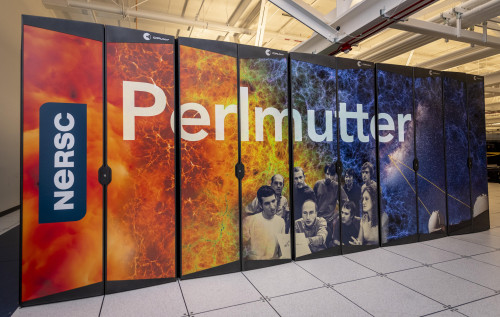
\includegraphics[width=0.5\textwidth]
    {images/perlmutter.jpg}
 \end{center}
\end{figure}

In addition to providing world-class supercomputers, NERSC offers expert support to ensure that its users make the most efficient and effective use of the facility's resources. NERSC staff help users optimize their applications for advanced computing architectures, and they engage with users from experimental facilities to run complex workflows on NERSC systems. Increasingly, NERSC staff aid users in implementing advanced analytics and machine learning capabilities into their applications and workflows. 

In 2021 NERSC unveiled its newest flagship supercomputer, Perlmutter, a Cray Shasta system based on NVIDIA A100 GPUs with new tensor core technology, AMD EPYC CPUs, and the HPE Cray ``Slingshot'' high-speed interconnect. The system is named in honor of Saul Perlmutter, an astrophysicist at Berkeley Lab and a professor of physics at UC Berkeley who shared the 2011 Nobel Prize in Physics for his contributions to research showing that the expansion of the universe is accelerating. Perlmutter is ranked as the 5th most powerful supercomputer in the world as of November 2021 and includes several innovations designed to meet the diverse computational and data analysis needs of NERSC's user base and speed their scientific productivity, including  an all-flash scratch filesystem. Developed by Cray to accelerate I/O, the 30-petabyte Lustre filesystem will move data at a rate of more than 4 terabytes/sec. 

\begin{figure}[h]
 \begin{center}
    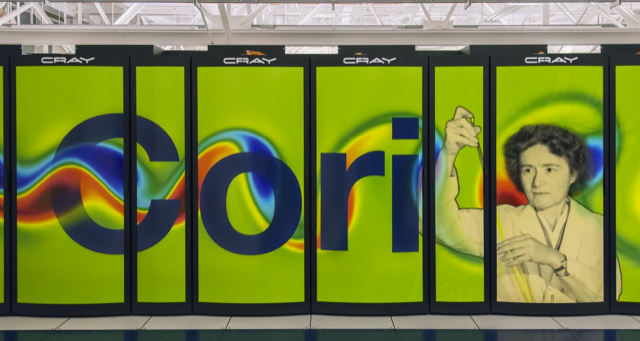
\includegraphics[width=0.6\textwidth]
    {images/cori.png}
 \end{center}
\end{figure}

NERSC also hosts an Intel-based Cray XC40 with a peak performance of 30 petaflop/s. Named ``Cori'' in honor of biochemist Gerty Cori, the first American woman to receive a Nobel Prize in science, the system delivered over 9 billion core hours in 2020 to the DOE SC user community and has several features that benefit data-intensive science. The system includes more than 1,600 Intel Xeon ``Haswell'' compute nodes and over 9,300 nodes of the Intel Xeon Phi processors (code-named Knights Landing, or KNL for short.  Cori uses the Cray Aries interconnect, a dragonfly network topology that provides scalable bandwidth.


NERSC has several storage platforms, including the Community Filesystem, a global file system available on all NERSC computational systems. It offers users a platform for collaboration and data sharing. NERSC systems are also connected to a High Performance Storage System (HPSS) for archival storage. NERSC's HPSS system currently contains more than 200 petabytes, making it one of the world's largest unclassified archival storage systems.


\subsubsection*{ESnet}

\begin{figure}[h]
  \begin{center}
    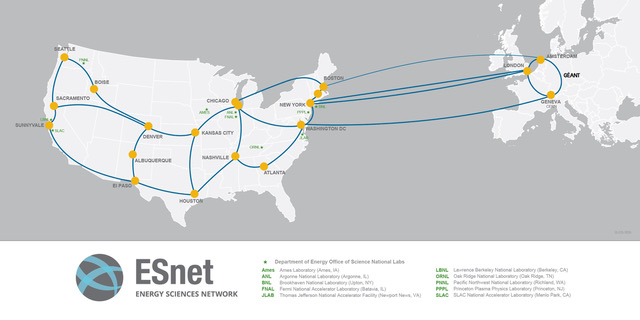
\includegraphics[width=0.95\textwidth]
    {images/esnet.jpeg}
  \end{center}
\end{figure}

ESnet interconnects the DOE's national laboratory system, dozens
of other DOE sites, and ~200 research and commercial networks around
the world, enabling tens of thousands of scientists at DOE laboratories
and academic institutions across the country to transfer vast data
streams and access distributed research and computing resources in
real-time. ESnet achieves this by providing high-bandwidth, reliable
connections that enable many thousands of the nation's scientists
to collaborate on some of the world's most important scientific
challenges including energy, biosciences, materials, and the origins
of the universe. ESnet operates what is essentially the Department's
circulatory system for the movement of large-scale scientific data,
providing real-time networking to many thousands of users across
the entire DOE complex.

Access to Berkeley Lab's computational and experimental facilities
from anywhere in the U.S.~or the world is provided by ESnet. ESnet
has extended its connectivity to Europe with four 100-Gbps connections.

\end{document}

%%% Local Variables:
%%% mode: latex
%%% TeX-master: t
%%% TeX-master: t
%%% End:
